\documentclass[twoside]{book}

% Packages required by doxygen
\usepackage{fixltx2e}
\usepackage{calc}
\usepackage{doxygen}
\usepackage[export]{adjustbox} % also loads graphicx
\usepackage{graphicx}
\usepackage[utf8]{inputenc}
\usepackage{makeidx}
\usepackage{multicol}
\usepackage{multirow}
\PassOptionsToPackage{warn}{textcomp}
\usepackage{textcomp}
\usepackage[nointegrals]{wasysym}
\usepackage[table]{xcolor}

% Font selection
\usepackage[T1]{fontenc}
\usepackage[scaled=.90]{helvet}
\usepackage{courier}
\usepackage{amssymb}
\usepackage{sectsty}
\renewcommand{\familydefault}{\sfdefault}
\allsectionsfont{%
  \fontseries{bc}\selectfont%
  \color{darkgray}%
}
\renewcommand{\DoxyLabelFont}{%
  \fontseries{bc}\selectfont%
  \color{darkgray}%
}
\newcommand{\+}{\discretionary{\mbox{\scriptsize$\hookleftarrow$}}{}{}}

% Page & text layout
\usepackage{geometry}
\geometry{%
  a4paper,%
  top=2.5cm,%
  bottom=2.5cm,%
  left=2.5cm,%
  right=2.5cm%
}
\tolerance=750
\hfuzz=15pt
\hbadness=750
\setlength{\emergencystretch}{15pt}
\setlength{\parindent}{0cm}
\setlength{\parskip}{3ex plus 2ex minus 2ex}
\makeatletter
\renewcommand{\paragraph}{%
  \@startsection{paragraph}{4}{0ex}{-1.0ex}{1.0ex}{%
    \normalfont\normalsize\bfseries\SS@parafont%
  }%
}
\renewcommand{\subparagraph}{%
  \@startsection{subparagraph}{5}{0ex}{-1.0ex}{1.0ex}{%
    \normalfont\normalsize\bfseries\SS@subparafont%
  }%
}
\makeatother

% Headers & footers
\usepackage{fancyhdr}
\pagestyle{fancyplain}
\fancyhead[LE]{\fancyplain{}{\bfseries\thepage}}
\fancyhead[CE]{\fancyplain{}{}}
\fancyhead[RE]{\fancyplain{}{\bfseries\leftmark}}
\fancyhead[LO]{\fancyplain{}{\bfseries\rightmark}}
\fancyhead[CO]{\fancyplain{}{}}
\fancyhead[RO]{\fancyplain{}{\bfseries\thepage}}
\fancyfoot[LE]{\fancyplain{}{}}
\fancyfoot[CE]{\fancyplain{}{}}
\fancyfoot[RE]{\fancyplain{}{\bfseries\scriptsize Generated by Doxygen }}
\fancyfoot[LO]{\fancyplain{}{\bfseries\scriptsize Generated by Doxygen }}
\fancyfoot[CO]{\fancyplain{}{}}
\fancyfoot[RO]{\fancyplain{}{}}
\renewcommand{\footrulewidth}{0.4pt}
\renewcommand{\chaptermark}[1]{%
  \markboth{#1}{}%
}
\renewcommand{\sectionmark}[1]{%
  \markright{\thesection\ #1}%
}

% Indices & bibliography
\usepackage{natbib}
\usepackage[titles]{tocloft}
\setcounter{tocdepth}{3}
\setcounter{secnumdepth}{5}
\makeindex

% Hyperlinks (required, but should be loaded last)
\usepackage{ifpdf}
\ifpdf
  \usepackage[pdftex,pagebackref=true]{hyperref}
\else
  \usepackage[ps2pdf,pagebackref=true]{hyperref}
\fi
\hypersetup{%
  colorlinks=true,%
  linkcolor=blue,%
  citecolor=blue,%
  unicode%
}

% Custom commands
\newcommand{\clearemptydoublepage}{%
  \newpage{\pagestyle{empty}\cleardoublepage}%
}

\usepackage{caption}
\captionsetup{labelsep=space,justification=centering,font={bf},singlelinecheck=off,skip=4pt,position=top}

%===== C O N T E N T S =====

\begin{document}

% Titlepage & ToC
\hypersetup{pageanchor=false,
             bookmarksnumbered=true,
             pdfencoding=unicode
            }
\pagenumbering{alph}
\begin{titlepage}
\vspace*{7cm}
\begin{center}%
{\Large My Project }\\
\vspace*{1cm}
{\large Generated by Doxygen 1.8.13}\\
\end{center}
\end{titlepage}
\clearemptydoublepage
\pagenumbering{roman}
\tableofcontents
\clearemptydoublepage
\pagenumbering{arabic}
\hypersetup{pageanchor=true}

%--- Begin generated contents ---
\chapter{Hierarchical Index}
\section{Class Hierarchy}
This inheritance list is sorted roughly, but not completely, alphabetically\+:\begin{DoxyCompactList}
\item \contentsline{section}{Client}{\pageref{classClient}}{}
\item \contentsline{section}{Game\+Mech}{\pageref{classGameMech}}{}
\item \contentsline{section}{Grid}{\pageref{classGrid}}{}
\item \contentsline{section}{Gui}{\pageref{classGui}}{}
\item \contentsline{section}{Player}{\pageref{classPlayer}}{}
\begin{DoxyCompactList}
\item \contentsline{section}{Bot\+Ai}{\pageref{classBotAi}}{}
\item \contentsline{section}{User}{\pageref{classUser}}{}
\end{DoxyCompactList}
\item \contentsline{section}{Server}{\pageref{classServer}}{}
\item \contentsline{section}{Ship}{\pageref{classShip}}{}
\item \contentsline{section}{Square}{\pageref{classSquare}}{}
\end{DoxyCompactList}

\chapter{Class Index}
\section{Class List}
Here are the classes, structs, unions and interfaces with brief descriptions\+:\begin{DoxyCompactList}
\item\contentsline{section}{\hyperlink{classBotAi}{Bot\+Ai} }{\pageref{classBotAi}}{}
\item\contentsline{section}{\hyperlink{classClient}{Client} }{\pageref{classClient}}{}
\item\contentsline{section}{\hyperlink{classGameMech}{Game\+Mech} }{\pageref{classGameMech}}{}
\item\contentsline{section}{\hyperlink{classGrid}{Grid} }{\pageref{classGrid}}{}
\item\contentsline{section}{\hyperlink{classGui}{Gui} }{\pageref{classGui}}{}
\item\contentsline{section}{\hyperlink{classPlayer}{Player} }{\pageref{classPlayer}}{}
\item\contentsline{section}{\hyperlink{classServer}{Server} }{\pageref{classServer}}{}
\item\contentsline{section}{\hyperlink{classShip}{Ship} }{\pageref{classShip}}{}
\item\contentsline{section}{\hyperlink{classSquare}{Square} }{\pageref{classSquare}}{}
\item\contentsline{section}{\hyperlink{classUser}{User} }{\pageref{classUser}}{}
\end{DoxyCompactList}

\chapter{Class Documentation}
\hypertarget{classbattleship_1_1game__server_1_1client}{}\section{battleship\+:\+:game\+\_\+server\+:\+:client Class Reference}
\label{classbattleship_1_1game__server_1_1client}\index{battleship\+::game\+\_\+server\+::client@{battleship\+::game\+\_\+server\+::client}}


Represents a client connected to the server.  




{\ttfamily \#include $<$client.\+h$>$}

\subsection*{Public Member Functions}
\begin{DoxyCompactItemize}
\item 
virtual \hyperlink{classbattleship_1_1game__server_1_1client_ac64f89eb976af431e4822dd777bdf320}{$\sim$client} ()
\item 
\hyperlink{classbattleship_1_1network__message_1_1message}{message} $\ast$ \hyperlink{classbattleship_1_1game__server_1_1client_a9824ce38f2f62979bd307487c862db9f}{receive} (const int tout\+\_\+s=0, const int tout\+\_\+us=0) const
\item 
ssize\+\_\+t \hyperlink{classbattleship_1_1game__server_1_1client_a9595ac710bf75e615afeee2a463a0872}{send} (const \hyperlink{classbattleship_1_1network__message_1_1message}{network\+\_\+message\+::message} $\ast$msg)
\item 
ssize\+\_\+t \hyperlink{classbattleship_1_1game__server_1_1client_a53b00e5370ae2f161784172eab1a9fdc}{send} (const \hyperlink{classbattleship_1_1network__message_1_1message}{network\+\_\+message\+::message} \&\&msg)
\item 
ssize\+\_\+t \hyperlink{classbattleship_1_1game__server_1_1client_a1aec51b5386354c5acd2b7a45486f7cc}{send} (const \hyperlink{classbattleship_1_1network__message_1_1message}{network\+\_\+message\+::message} \&msg)
\item 
unsigned char \hyperlink{classbattleship_1_1game__server_1_1client_ac1427b1a3a9dd9f2a0185b6c0d36e1c5}{get\+\_\+id} ()
\item 
const unsigned char \hyperlink{classbattleship_1_1game__server_1_1client_a2829c94437fea654b900dc801750d8ef}{get\+\_\+id} () const
\item 
std\+::string \hyperlink{classbattleship_1_1game__server_1_1client_abb6392156781049b20f0e7490da49840}{get\+\_\+name} ()
\item 
const std\+::string \hyperlink{classbattleship_1_1game__server_1_1client_ab10f638915409ca61ee52838c476e89c}{get\+\_\+name} () const
\item 
unsigned char \hyperlink{classbattleship_1_1game__server_1_1client_a232605975d752a2d5a30a606c5b890c6}{get\+\_\+game\+\_\+id} ()
\item 
const unsigned char \hyperlink{classbattleship_1_1game__server_1_1client_a6152f49fe5202ff8b9bd249071c03406}{get\+\_\+game\+\_\+id} () const
\item 
void \hyperlink{classbattleship_1_1game__server_1_1client_adfd1858da78c5ad2aba9a5528190882b}{set\+\_\+in\+\_\+game} (const char g\+\_\+id)
\item 
bool \hyperlink{classbattleship_1_1game__server_1_1client_ad985a33f008c3c16dbb1a244cabe32db}{is\+\_\+in\+\_\+game} ()
\item 
const bool \hyperlink{classbattleship_1_1game__server_1_1client_a3d2b688869f4470381cd47f09d8a6239}{is\+\_\+in\+\_\+game} () const
\item 
void \hyperlink{classbattleship_1_1game__server_1_1client_a106984508ae941fa5a88dbe066214ad4}{set\+\_\+idle} ()
\item 
bool \hyperlink{classbattleship_1_1game__server_1_1client_a0f8168fdcc8e5ff4daa41eb208173a1a}{is\+\_\+idle} ()
\item 
const bool \hyperlink{classbattleship_1_1game__server_1_1client_a996d6df89391d08aa4b02d7a2ae77322}{is\+\_\+idle} () const
\item 
void \hyperlink{classbattleship_1_1game__server_1_1client_abee4c579c35854d0a79a1f0dbc712006}{set\+\_\+searching} ()
\item 
bool \hyperlink{classbattleship_1_1game__server_1_1client_a0a95758fec7cd830ca19278a2b619e92}{is\+\_\+searching} ()
\item 
const bool \hyperlink{classbattleship_1_1game__server_1_1client_a6438e71d667d166f663d8d7e67ff7d38}{is\+\_\+searching} () const
\item 
bool \hyperlink{classbattleship_1_1game__server_1_1client_a3975d4198aa55bdf690e2268b3f76080}{timed\+\_\+out} (const int max\+\_\+touts)
\item 
void \hyperlink{classbattleship_1_1game__server_1_1client_a8f594fcecac15941f7fee46a0340bfe4}{reset\+\_\+timeouts} ()
\item 
std\+::string \hyperlink{classbattleship_1_1game__server_1_1client_a828c6732dc5e35bd2cfd1f73d69a54a9}{get\+\_\+listing} ()
\end{DoxyCompactItemize}
\subsection*{Friends}
\begin{DoxyCompactItemize}
\item 
\mbox{\Hypertarget{classbattleship_1_1game__server_1_1client_ab170f98a853909cd44b3f981a3c3aff5}\label{classbattleship_1_1game__server_1_1client_ab170f98a853909cd44b3f981a3c3aff5}} 
class {\bfseries client\+\_\+pool}
\end{DoxyCompactItemize}


\subsection{Detailed Description}
Represents a client connected to the server. 

\begin{DoxyAuthor}{Author}
Jonathan Henly 

Adham Kassem 
\end{DoxyAuthor}
\begin{DoxyVersion}{Version}
11-\/27-\/2018 
\end{DoxyVersion}


\subsection{Constructor \& Destructor Documentation}
\mbox{\Hypertarget{classbattleship_1_1game__server_1_1client_ac64f89eb976af431e4822dd777bdf320}\label{classbattleship_1_1game__server_1_1client_ac64f89eb976af431e4822dd777bdf320}} 
\index{battleship\+::game\+\_\+server\+::client@{battleship\+::game\+\_\+server\+::client}!````~client@{$\sim$client}}
\index{````~client@{$\sim$client}!battleship\+::game\+\_\+server\+::client@{battleship\+::game\+\_\+server\+::client}}
\subsubsection{\texorpdfstring{$\sim$client()}{~client()}}
{\footnotesize\ttfamily virtual battleship\+::game\+\_\+server\+::client\+::$\sim$client (\begin{DoxyParamCaption}{ }\end{DoxyParamCaption})\hspace{0.3cm}{\ttfamily [inline]}, {\ttfamily [virtual]}}

Destructor that deletes the
\begin{DoxyCode}
\hyperlink{classtcp__stream}{tcp\_stream} 
\end{DoxyCode}
 connection associated with this server client. 

\subsection{Member Function Documentation}
\mbox{\Hypertarget{classbattleship_1_1game__server_1_1client_a232605975d752a2d5a30a606c5b890c6}\label{classbattleship_1_1game__server_1_1client_a232605975d752a2d5a30a606c5b890c6}} 
\index{battleship\+::game\+\_\+server\+::client@{battleship\+::game\+\_\+server\+::client}!get\+\_\+game\+\_\+id@{get\+\_\+game\+\_\+id}}
\index{get\+\_\+game\+\_\+id@{get\+\_\+game\+\_\+id}!battleship\+::game\+\_\+server\+::client@{battleship\+::game\+\_\+server\+::client}}
\subsubsection{\texorpdfstring{get\+\_\+game\+\_\+id()}{get\_game\_id()}\hspace{0.1cm}{\footnotesize\ttfamily [1/2]}}
{\footnotesize\ttfamily unsigned char battleship\+::game\+\_\+server\+::client\+::get\+\_\+game\+\_\+id (\begin{DoxyParamCaption}{ }\end{DoxyParamCaption})\hspace{0.3cm}{\ttfamily [inline]}}

\begin{DoxyReturn}{Returns}
the ID of the game this client is in, or 0. 
\end{DoxyReturn}
\mbox{\Hypertarget{classbattleship_1_1game__server_1_1client_a6152f49fe5202ff8b9bd249071c03406}\label{classbattleship_1_1game__server_1_1client_a6152f49fe5202ff8b9bd249071c03406}} 
\index{battleship\+::game\+\_\+server\+::client@{battleship\+::game\+\_\+server\+::client}!get\+\_\+game\+\_\+id@{get\+\_\+game\+\_\+id}}
\index{get\+\_\+game\+\_\+id@{get\+\_\+game\+\_\+id}!battleship\+::game\+\_\+server\+::client@{battleship\+::game\+\_\+server\+::client}}
\subsubsection{\texorpdfstring{get\+\_\+game\+\_\+id()}{get\_game\_id()}\hspace{0.1cm}{\footnotesize\ttfamily [2/2]}}
{\footnotesize\ttfamily const unsigned char battleship\+::game\+\_\+server\+::client\+::get\+\_\+game\+\_\+id (\begin{DoxyParamCaption}{ }\end{DoxyParamCaption}) const\hspace{0.3cm}{\ttfamily [inline]}}

\begin{DoxyReturn}{Returns}
the ID of the game this client is in, or 0. 
\end{DoxyReturn}
\mbox{\Hypertarget{classbattleship_1_1game__server_1_1client_ac1427b1a3a9dd9f2a0185b6c0d36e1c5}\label{classbattleship_1_1game__server_1_1client_ac1427b1a3a9dd9f2a0185b6c0d36e1c5}} 
\index{battleship\+::game\+\_\+server\+::client@{battleship\+::game\+\_\+server\+::client}!get\+\_\+id@{get\+\_\+id}}
\index{get\+\_\+id@{get\+\_\+id}!battleship\+::game\+\_\+server\+::client@{battleship\+::game\+\_\+server\+::client}}
\subsubsection{\texorpdfstring{get\+\_\+id()}{get\_id()}\hspace{0.1cm}{\footnotesize\ttfamily [1/2]}}
{\footnotesize\ttfamily unsigned char battleship\+::game\+\_\+server\+::client\+::get\+\_\+id (\begin{DoxyParamCaption}{ }\end{DoxyParamCaption})\hspace{0.3cm}{\ttfamily [inline]}}

\begin{DoxyReturn}{Returns}
this client\textquotesingle{}s ID. 
\end{DoxyReturn}
\mbox{\Hypertarget{classbattleship_1_1game__server_1_1client_a2829c94437fea654b900dc801750d8ef}\label{classbattleship_1_1game__server_1_1client_a2829c94437fea654b900dc801750d8ef}} 
\index{battleship\+::game\+\_\+server\+::client@{battleship\+::game\+\_\+server\+::client}!get\+\_\+id@{get\+\_\+id}}
\index{get\+\_\+id@{get\+\_\+id}!battleship\+::game\+\_\+server\+::client@{battleship\+::game\+\_\+server\+::client}}
\subsubsection{\texorpdfstring{get\+\_\+id()}{get\_id()}\hspace{0.1cm}{\footnotesize\ttfamily [2/2]}}
{\footnotesize\ttfamily const unsigned char battleship\+::game\+\_\+server\+::client\+::get\+\_\+id (\begin{DoxyParamCaption}{ }\end{DoxyParamCaption}) const\hspace{0.3cm}{\ttfamily [inline]}}

\begin{DoxyReturn}{Returns}
this client\textquotesingle{}s ID. 
\end{DoxyReturn}
\mbox{\Hypertarget{classbattleship_1_1game__server_1_1client_a828c6732dc5e35bd2cfd1f73d69a54a9}\label{classbattleship_1_1game__server_1_1client_a828c6732dc5e35bd2cfd1f73d69a54a9}} 
\index{battleship\+::game\+\_\+server\+::client@{battleship\+::game\+\_\+server\+::client}!get\+\_\+listing@{get\+\_\+listing}}
\index{get\+\_\+listing@{get\+\_\+listing}!battleship\+::game\+\_\+server\+::client@{battleship\+::game\+\_\+server\+::client}}
\subsubsection{\texorpdfstring{get\+\_\+listing()}{get\_listing()}}
{\footnotesize\ttfamily std\+::string battleship\+::game\+\_\+server\+::client\+::get\+\_\+listing (\begin{DoxyParamCaption}{ }\end{DoxyParamCaption})\hspace{0.3cm}{\ttfamily [inline]}}

Returns this client\textquotesingle{}s listing as an
\begin{DoxyCode}
std::string 
\end{DoxyCode}
 . The first 
\begin{DoxyCode}
\textcolor{keywordtype}{char} 
\end{DoxyCode}
 is the client\textquotesingle{}s ID, the second is the client\textquotesingle{}s status and

\begin{DoxyReturn}{Returns}

\end{DoxyReturn}
\mbox{\Hypertarget{classbattleship_1_1game__server_1_1client_abb6392156781049b20f0e7490da49840}\label{classbattleship_1_1game__server_1_1client_abb6392156781049b20f0e7490da49840}} 
\index{battleship\+::game\+\_\+server\+::client@{battleship\+::game\+\_\+server\+::client}!get\+\_\+name@{get\+\_\+name}}
\index{get\+\_\+name@{get\+\_\+name}!battleship\+::game\+\_\+server\+::client@{battleship\+::game\+\_\+server\+::client}}
\subsubsection{\texorpdfstring{get\+\_\+name()}{get\_name()}\hspace{0.1cm}{\footnotesize\ttfamily [1/2]}}
{\footnotesize\ttfamily std\+::string battleship\+::game\+\_\+server\+::client\+::get\+\_\+name (\begin{DoxyParamCaption}{ }\end{DoxyParamCaption})\hspace{0.3cm}{\ttfamily [inline]}}

\begin{DoxyReturn}{Returns}
this client\textquotesingle{}s name. 
\end{DoxyReturn}
\mbox{\Hypertarget{classbattleship_1_1game__server_1_1client_ab10f638915409ca61ee52838c476e89c}\label{classbattleship_1_1game__server_1_1client_ab10f638915409ca61ee52838c476e89c}} 
\index{battleship\+::game\+\_\+server\+::client@{battleship\+::game\+\_\+server\+::client}!get\+\_\+name@{get\+\_\+name}}
\index{get\+\_\+name@{get\+\_\+name}!battleship\+::game\+\_\+server\+::client@{battleship\+::game\+\_\+server\+::client}}
\subsubsection{\texorpdfstring{get\+\_\+name()}{get\_name()}\hspace{0.1cm}{\footnotesize\ttfamily [2/2]}}
{\footnotesize\ttfamily const std\+::string battleship\+::game\+\_\+server\+::client\+::get\+\_\+name (\begin{DoxyParamCaption}{ }\end{DoxyParamCaption}) const\hspace{0.3cm}{\ttfamily [inline]}}

\begin{DoxyReturn}{Returns}
this client\textquotesingle{}s name. 
\end{DoxyReturn}
\mbox{\Hypertarget{classbattleship_1_1game__server_1_1client_a0f8168fdcc8e5ff4daa41eb208173a1a}\label{classbattleship_1_1game__server_1_1client_a0f8168fdcc8e5ff4daa41eb208173a1a}} 
\index{battleship\+::game\+\_\+server\+::client@{battleship\+::game\+\_\+server\+::client}!is\+\_\+idle@{is\+\_\+idle}}
\index{is\+\_\+idle@{is\+\_\+idle}!battleship\+::game\+\_\+server\+::client@{battleship\+::game\+\_\+server\+::client}}
\subsubsection{\texorpdfstring{is\+\_\+idle()}{is\_idle()}\hspace{0.1cm}{\footnotesize\ttfamily [1/2]}}
{\footnotesize\ttfamily bool battleship\+::game\+\_\+server\+::client\+::is\+\_\+idle (\begin{DoxyParamCaption}{ }\end{DoxyParamCaption})\hspace{0.3cm}{\ttfamily [inline]}}

\begin{DoxyReturn}{Returns}
true if the status of this client is idle, false otherwise. 
\end{DoxyReturn}
\mbox{\Hypertarget{classbattleship_1_1game__server_1_1client_a996d6df89391d08aa4b02d7a2ae77322}\label{classbattleship_1_1game__server_1_1client_a996d6df89391d08aa4b02d7a2ae77322}} 
\index{battleship\+::game\+\_\+server\+::client@{battleship\+::game\+\_\+server\+::client}!is\+\_\+idle@{is\+\_\+idle}}
\index{is\+\_\+idle@{is\+\_\+idle}!battleship\+::game\+\_\+server\+::client@{battleship\+::game\+\_\+server\+::client}}
\subsubsection{\texorpdfstring{is\+\_\+idle()}{is\_idle()}\hspace{0.1cm}{\footnotesize\ttfamily [2/2]}}
{\footnotesize\ttfamily const bool battleship\+::game\+\_\+server\+::client\+::is\+\_\+idle (\begin{DoxyParamCaption}{ }\end{DoxyParamCaption}) const\hspace{0.3cm}{\ttfamily [inline]}}

\begin{DoxyReturn}{Returns}
true if the status of this client is idle, false otherwise. 
\end{DoxyReturn}
\mbox{\Hypertarget{classbattleship_1_1game__server_1_1client_ad985a33f008c3c16dbb1a244cabe32db}\label{classbattleship_1_1game__server_1_1client_ad985a33f008c3c16dbb1a244cabe32db}} 
\index{battleship\+::game\+\_\+server\+::client@{battleship\+::game\+\_\+server\+::client}!is\+\_\+in\+\_\+game@{is\+\_\+in\+\_\+game}}
\index{is\+\_\+in\+\_\+game@{is\+\_\+in\+\_\+game}!battleship\+::game\+\_\+server\+::client@{battleship\+::game\+\_\+server\+::client}}
\subsubsection{\texorpdfstring{is\+\_\+in\+\_\+game()}{is\_in\_game()}\hspace{0.1cm}{\footnotesize\ttfamily [1/2]}}
{\footnotesize\ttfamily bool battleship\+::game\+\_\+server\+::client\+::is\+\_\+in\+\_\+game (\begin{DoxyParamCaption}{ }\end{DoxyParamCaption})\hspace{0.3cm}{\ttfamily [inline]}}

\begin{DoxyReturn}{Returns}
true if the status of this client is in-\/game, false otherwise. 
\end{DoxyReturn}
\mbox{\Hypertarget{classbattleship_1_1game__server_1_1client_a3d2b688869f4470381cd47f09d8a6239}\label{classbattleship_1_1game__server_1_1client_a3d2b688869f4470381cd47f09d8a6239}} 
\index{battleship\+::game\+\_\+server\+::client@{battleship\+::game\+\_\+server\+::client}!is\+\_\+in\+\_\+game@{is\+\_\+in\+\_\+game}}
\index{is\+\_\+in\+\_\+game@{is\+\_\+in\+\_\+game}!battleship\+::game\+\_\+server\+::client@{battleship\+::game\+\_\+server\+::client}}
\subsubsection{\texorpdfstring{is\+\_\+in\+\_\+game()}{is\_in\_game()}\hspace{0.1cm}{\footnotesize\ttfamily [2/2]}}
{\footnotesize\ttfamily const bool battleship\+::game\+\_\+server\+::client\+::is\+\_\+in\+\_\+game (\begin{DoxyParamCaption}{ }\end{DoxyParamCaption}) const\hspace{0.3cm}{\ttfamily [inline]}}

\begin{DoxyReturn}{Returns}
true if the status of this client is in-\/game, false otherwise. 
\end{DoxyReturn}
\mbox{\Hypertarget{classbattleship_1_1game__server_1_1client_a0a95758fec7cd830ca19278a2b619e92}\label{classbattleship_1_1game__server_1_1client_a0a95758fec7cd830ca19278a2b619e92}} 
\index{battleship\+::game\+\_\+server\+::client@{battleship\+::game\+\_\+server\+::client}!is\+\_\+searching@{is\+\_\+searching}}
\index{is\+\_\+searching@{is\+\_\+searching}!battleship\+::game\+\_\+server\+::client@{battleship\+::game\+\_\+server\+::client}}
\subsubsection{\texorpdfstring{is\+\_\+searching()}{is\_searching()}\hspace{0.1cm}{\footnotesize\ttfamily [1/2]}}
{\footnotesize\ttfamily bool battleship\+::game\+\_\+server\+::client\+::is\+\_\+searching (\begin{DoxyParamCaption}{ }\end{DoxyParamCaption})\hspace{0.3cm}{\ttfamily [inline]}}

\begin{DoxyReturn}{Returns}
true if the status of this client is busy, false otherwise. 
\end{DoxyReturn}
\mbox{\Hypertarget{classbattleship_1_1game__server_1_1client_a6438e71d667d166f663d8d7e67ff7d38}\label{classbattleship_1_1game__server_1_1client_a6438e71d667d166f663d8d7e67ff7d38}} 
\index{battleship\+::game\+\_\+server\+::client@{battleship\+::game\+\_\+server\+::client}!is\+\_\+searching@{is\+\_\+searching}}
\index{is\+\_\+searching@{is\+\_\+searching}!battleship\+::game\+\_\+server\+::client@{battleship\+::game\+\_\+server\+::client}}
\subsubsection{\texorpdfstring{is\+\_\+searching()}{is\_searching()}\hspace{0.1cm}{\footnotesize\ttfamily [2/2]}}
{\footnotesize\ttfamily const bool battleship\+::game\+\_\+server\+::client\+::is\+\_\+searching (\begin{DoxyParamCaption}{ }\end{DoxyParamCaption}) const\hspace{0.3cm}{\ttfamily [inline]}}

\begin{DoxyReturn}{Returns}
true if the status of this client is busy, false otherwise. 
\end{DoxyReturn}
\mbox{\Hypertarget{classbattleship_1_1game__server_1_1client_a9824ce38f2f62979bd307487c862db9f}\label{classbattleship_1_1game__server_1_1client_a9824ce38f2f62979bd307487c862db9f}} 
\index{battleship\+::game\+\_\+server\+::client@{battleship\+::game\+\_\+server\+::client}!receive@{receive}}
\index{receive@{receive}!battleship\+::game\+\_\+server\+::client@{battleship\+::game\+\_\+server\+::client}}
\subsubsection{\texorpdfstring{receive()}{receive()}}
{\footnotesize\ttfamily \hyperlink{classbattleship_1_1network__message_1_1message}{message}$\ast$ battleship\+::game\+\_\+server\+::client\+::receive (\begin{DoxyParamCaption}\item[{const int}]{tout\+\_\+s = {\ttfamily 0},  }\item[{const int}]{tout\+\_\+us = {\ttfamily 0} }\end{DoxyParamCaption}) const\hspace{0.3cm}{\ttfamily [inline]}}

Returns a pointer to a message that was created from the bytes sent by this client.

Note\+: if both
\begin{DoxyCode}
tout\_s 
\end{DoxyCode}
 and
\begin{DoxyCode}
tout\_us 
\end{DoxyCode}
 are 0, the this method will block until data is received.


\begin{DoxyParams}{Parameters}
{\em tout\+\_\+s} & -\/ the time to wait for data in seconds. \\
\hline
{\em tout\+\_\+us} & -\/ the time to wait for data in microseconds. \\
\hline
\end{DoxyParams}
\begin{DoxyReturn}{Returns}
a pointer to a message constructed from the bytes this client sent. 
\end{DoxyReturn}
\mbox{\Hypertarget{classbattleship_1_1game__server_1_1client_a8f594fcecac15941f7fee46a0340bfe4}\label{classbattleship_1_1game__server_1_1client_a8f594fcecac15941f7fee46a0340bfe4}} 
\index{battleship\+::game\+\_\+server\+::client@{battleship\+::game\+\_\+server\+::client}!reset\+\_\+timeouts@{reset\+\_\+timeouts}}
\index{reset\+\_\+timeouts@{reset\+\_\+timeouts}!battleship\+::game\+\_\+server\+::client@{battleship\+::game\+\_\+server\+::client}}
\subsubsection{\texorpdfstring{reset\+\_\+timeouts()}{reset\_timeouts()}}
{\footnotesize\ttfamily void battleship\+::game\+\_\+server\+::client\+::reset\+\_\+timeouts (\begin{DoxyParamCaption}{ }\end{DoxyParamCaption})\hspace{0.3cm}{\ttfamily [inline]}}

Resets this client\textquotesingle{}s timeout count to zero. \mbox{\Hypertarget{classbattleship_1_1game__server_1_1client_a9595ac710bf75e615afeee2a463a0872}\label{classbattleship_1_1game__server_1_1client_a9595ac710bf75e615afeee2a463a0872}} 
\index{battleship\+::game\+\_\+server\+::client@{battleship\+::game\+\_\+server\+::client}!send@{send}}
\index{send@{send}!battleship\+::game\+\_\+server\+::client@{battleship\+::game\+\_\+server\+::client}}
\subsubsection{\texorpdfstring{send()}{send()}\hspace{0.1cm}{\footnotesize\ttfamily [1/3]}}
{\footnotesize\ttfamily ssize\+\_\+t battleship\+::game\+\_\+server\+::client\+::send (\begin{DoxyParamCaption}\item[{const \hyperlink{classbattleship_1_1network__message_1_1message}{network\+\_\+message\+::message} $\ast$}]{msg }\end{DoxyParamCaption})\hspace{0.3cm}{\ttfamily [inline]}}

Sends a message over the network to a client.


\begin{DoxyParams}{Parameters}
{\em msg} & -\/ a pointer to the message to send to the client.\\
\hline
\end{DoxyParams}
\begin{DoxyReturn}{Returns}
the number of bytes sent to the client, or if negative, an error value. 
\end{DoxyReturn}
\mbox{\Hypertarget{classbattleship_1_1game__server_1_1client_a53b00e5370ae2f161784172eab1a9fdc}\label{classbattleship_1_1game__server_1_1client_a53b00e5370ae2f161784172eab1a9fdc}} 
\index{battleship\+::game\+\_\+server\+::client@{battleship\+::game\+\_\+server\+::client}!send@{send}}
\index{send@{send}!battleship\+::game\+\_\+server\+::client@{battleship\+::game\+\_\+server\+::client}}
\subsubsection{\texorpdfstring{send()}{send()}\hspace{0.1cm}{\footnotesize\ttfamily [2/3]}}
{\footnotesize\ttfamily ssize\+\_\+t battleship\+::game\+\_\+server\+::client\+::send (\begin{DoxyParamCaption}\item[{const \hyperlink{classbattleship_1_1network__message_1_1message}{network\+\_\+message\+::message} \&\&}]{msg }\end{DoxyParamCaption})\hspace{0.3cm}{\ttfamily [inline]}}

Sends a message over the network to a client.


\begin{DoxyParams}{Parameters}
{\em msg} & -\/ the message to send to the client.\\
\hline
\end{DoxyParams}
\begin{DoxyReturn}{Returns}
the number of bytes sent to the client, or if negative, an error value. 
\end{DoxyReturn}
\mbox{\Hypertarget{classbattleship_1_1game__server_1_1client_a1aec51b5386354c5acd2b7a45486f7cc}\label{classbattleship_1_1game__server_1_1client_a1aec51b5386354c5acd2b7a45486f7cc}} 
\index{battleship\+::game\+\_\+server\+::client@{battleship\+::game\+\_\+server\+::client}!send@{send}}
\index{send@{send}!battleship\+::game\+\_\+server\+::client@{battleship\+::game\+\_\+server\+::client}}
\subsubsection{\texorpdfstring{send()}{send()}\hspace{0.1cm}{\footnotesize\ttfamily [3/3]}}
{\footnotesize\ttfamily ssize\+\_\+t battleship\+::game\+\_\+server\+::client\+::send (\begin{DoxyParamCaption}\item[{const \hyperlink{classbattleship_1_1network__message_1_1message}{network\+\_\+message\+::message} \&}]{msg }\end{DoxyParamCaption})\hspace{0.3cm}{\ttfamily [inline]}}

Sends a message over the network to a client.


\begin{DoxyParams}{Parameters}
{\em msg} & -\/ the message to send to the client.\\
\hline
\end{DoxyParams}
\begin{DoxyReturn}{Returns}
the number of bytes sent to the client, or if negative, an error value. 
\end{DoxyReturn}
\mbox{\Hypertarget{classbattleship_1_1game__server_1_1client_a106984508ae941fa5a88dbe066214ad4}\label{classbattleship_1_1game__server_1_1client_a106984508ae941fa5a88dbe066214ad4}} 
\index{battleship\+::game\+\_\+server\+::client@{battleship\+::game\+\_\+server\+::client}!set\+\_\+idle@{set\+\_\+idle}}
\index{set\+\_\+idle@{set\+\_\+idle}!battleship\+::game\+\_\+server\+::client@{battleship\+::game\+\_\+server\+::client}}
\subsubsection{\texorpdfstring{set\+\_\+idle()}{set\_idle()}}
{\footnotesize\ttfamily void battleship\+::game\+\_\+server\+::client\+::set\+\_\+idle (\begin{DoxyParamCaption}{ }\end{DoxyParamCaption})\hspace{0.3cm}{\ttfamily [inline]}}

Sets the status of this client to idle. \mbox{\Hypertarget{classbattleship_1_1game__server_1_1client_adfd1858da78c5ad2aba9a5528190882b}\label{classbattleship_1_1game__server_1_1client_adfd1858da78c5ad2aba9a5528190882b}} 
\index{battleship\+::game\+\_\+server\+::client@{battleship\+::game\+\_\+server\+::client}!set\+\_\+in\+\_\+game@{set\+\_\+in\+\_\+game}}
\index{set\+\_\+in\+\_\+game@{set\+\_\+in\+\_\+game}!battleship\+::game\+\_\+server\+::client@{battleship\+::game\+\_\+server\+::client}}
\subsubsection{\texorpdfstring{set\+\_\+in\+\_\+game()}{set\_in\_game()}}
{\footnotesize\ttfamily void battleship\+::game\+\_\+server\+::client\+::set\+\_\+in\+\_\+game (\begin{DoxyParamCaption}\item[{const char}]{g\+\_\+id }\end{DoxyParamCaption})\hspace{0.3cm}{\ttfamily [inline]}}

Sets the status of this client to in-\/game. \mbox{\Hypertarget{classbattleship_1_1game__server_1_1client_abee4c579c35854d0a79a1f0dbc712006}\label{classbattleship_1_1game__server_1_1client_abee4c579c35854d0a79a1f0dbc712006}} 
\index{battleship\+::game\+\_\+server\+::client@{battleship\+::game\+\_\+server\+::client}!set\+\_\+searching@{set\+\_\+searching}}
\index{set\+\_\+searching@{set\+\_\+searching}!battleship\+::game\+\_\+server\+::client@{battleship\+::game\+\_\+server\+::client}}
\subsubsection{\texorpdfstring{set\+\_\+searching()}{set\_searching()}}
{\footnotesize\ttfamily void battleship\+::game\+\_\+server\+::client\+::set\+\_\+searching (\begin{DoxyParamCaption}{ }\end{DoxyParamCaption})\hspace{0.3cm}{\ttfamily [inline]}}

Sets the status of this client to busy. \mbox{\Hypertarget{classbattleship_1_1game__server_1_1client_a3975d4198aa55bdf690e2268b3f76080}\label{classbattleship_1_1game__server_1_1client_a3975d4198aa55bdf690e2268b3f76080}} 
\index{battleship\+::game\+\_\+server\+::client@{battleship\+::game\+\_\+server\+::client}!timed\+\_\+out@{timed\+\_\+out}}
\index{timed\+\_\+out@{timed\+\_\+out}!battleship\+::game\+\_\+server\+::client@{battleship\+::game\+\_\+server\+::client}}
\subsubsection{\texorpdfstring{timed\+\_\+out()}{timed\_out()}}
{\footnotesize\ttfamily bool battleship\+::game\+\_\+server\+::client\+::timed\+\_\+out (\begin{DoxyParamCaption}\item[{const int}]{max\+\_\+touts }\end{DoxyParamCaption})\hspace{0.3cm}{\ttfamily [inline]}}


\begin{DoxyParams}{Parameters}
{\em max\+\_\+touts} & -\/ the number of allowed timeouts before action should be taken. \\
\hline
\end{DoxyParams}
\begin{DoxyReturn}{Returns}
true if this client\textquotesingle{}s timeout count is greater than 
\begin{DoxyCode}
max\_touts 
\end{DoxyCode}
 , otherwise false. 
\end{DoxyReturn}


The documentation for this class was generated from the following file\+:\begin{DoxyCompactItemize}
\item 
inc/client.\+h\end{DoxyCompactItemize}

\hypertarget{classbattleship_1_1game__server_1_1client__message__producer}{}\section{battleship\+:\+:game\+\_\+server\+:\+:client\+\_\+message\+\_\+producer Class Reference}
\label{classbattleship_1_1game__server_1_1client__message__producer}\index{battleship\+::game\+\_\+server\+::client\+\_\+message\+\_\+producer@{battleship\+::game\+\_\+server\+::client\+\_\+message\+\_\+producer}}


Handles the connections between clients and the server.  




{\ttfamily \#include $<$msgproducer.\+h$>$}



Inheritance diagram for battleship\+:\+:game\+\_\+server\+:\+:client\+\_\+message\+\_\+producer\+:
\nopagebreak
\begin{figure}[H]
\begin{center}
\leavevmode
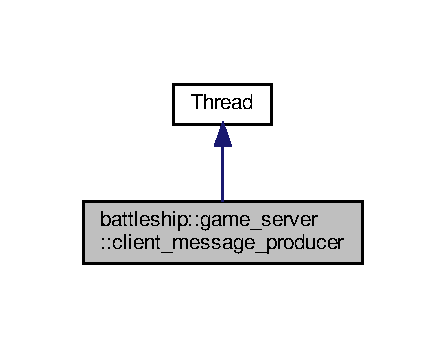
\includegraphics[width=214pt]{classbattleship_1_1game__server_1_1client__message__producer__inherit__graph}
\end{center}
\end{figure}


Collaboration diagram for battleship\+:\+:game\+\_\+server\+:\+:client\+\_\+message\+\_\+producer\+:
\nopagebreak
\begin{figure}[H]
\begin{center}
\leavevmode
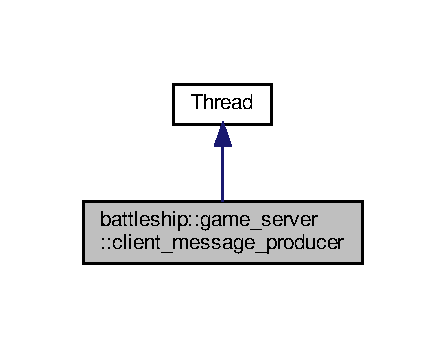
\includegraphics[width=214pt]{classbattleship_1_1game__server_1_1client__message__producer__coll__graph}
\end{center}
\end{figure}
\subsection*{Public Member Functions}
\begin{DoxyCompactItemize}
\item 
\hyperlink{classbattleship_1_1game__server_1_1client__message__producer_a5f2a0bfac369d551954a77c58c2abad2}{client\+\_\+message\+\_\+producer} (\hyperlink{classbattleship_1_1ts__queue}{ts\+\_\+queue}$<$ std\+::weak\+\_\+ptr$<$ \hyperlink{classbattleship_1_1game__server_1_1client}{client} $>$$>$ \&c\+\_\+queue, \hyperlink{classbattleship_1_1game__server_1_1client__pool}{client\+\_\+pool} \&c\+\_\+pool, \hyperlink{classbattleship_1_1ts__queue}{ts\+\_\+queue}$<$ \hyperlink{classbattleship_1_1network__message_1_1message}{message} $\ast$$>$ \&m\+\_\+queue, const unsigned int num\+\_\+timeout\+\_\+limit=30000)
\item 
\mbox{\Hypertarget{classbattleship_1_1game__server_1_1client__message__producer_af3f501bb1e23993e7958d990e44219ed}\label{classbattleship_1_1game__server_1_1client__message__producer_af3f501bb1e23993e7958d990e44219ed}} 
void $\ast$ {\bfseries run} () override
\end{DoxyCompactItemize}


\subsection{Detailed Description}
Handles the connections between clients and the server. 

\begin{DoxyAuthor}{Author}
Jonathan Henly 

Adham Kassem 
\end{DoxyAuthor}
\begin{DoxyVersion}{Version}
12-\/4-\/2018 
\end{DoxyVersion}


\subsection{Constructor \& Destructor Documentation}
\mbox{\Hypertarget{classbattleship_1_1game__server_1_1client__message__producer_a5f2a0bfac369d551954a77c58c2abad2}\label{classbattleship_1_1game__server_1_1client__message__producer_a5f2a0bfac369d551954a77c58c2abad2}} 
\index{battleship\+::game\+\_\+server\+::client\+\_\+message\+\_\+producer@{battleship\+::game\+\_\+server\+::client\+\_\+message\+\_\+producer}!client\+\_\+message\+\_\+producer@{client\+\_\+message\+\_\+producer}}
\index{client\+\_\+message\+\_\+producer@{client\+\_\+message\+\_\+producer}!battleship\+::game\+\_\+server\+::client\+\_\+message\+\_\+producer@{battleship\+::game\+\_\+server\+::client\+\_\+message\+\_\+producer}}
\subsubsection{\texorpdfstring{client\+\_\+message\+\_\+producer()}{client\_message\_producer()}}
{\footnotesize\ttfamily battleship\+::game\+\_\+server\+::client\+\_\+message\+\_\+producer\+::client\+\_\+message\+\_\+producer (\begin{DoxyParamCaption}\item[{\hyperlink{classbattleship_1_1ts__queue}{ts\+\_\+queue}$<$ std\+::weak\+\_\+ptr$<$ \hyperlink{classbattleship_1_1game__server_1_1client}{client} $>$$>$ \&}]{c\+\_\+queue,  }\item[{\hyperlink{classbattleship_1_1game__server_1_1client__pool}{client\+\_\+pool} \&}]{c\+\_\+pool,  }\item[{\hyperlink{classbattleship_1_1ts__queue}{ts\+\_\+queue}$<$ \hyperlink{classbattleship_1_1network__message_1_1message}{message} $\ast$$>$ \&}]{m\+\_\+queue,  }\item[{const unsigned int}]{num\+\_\+timeout\+\_\+limit = {\ttfamily 30000} }\end{DoxyParamCaption})\hspace{0.3cm}{\ttfamily [inline]}}


\begin{DoxyParams}{Parameters}
{\em c\+\_\+queue} & \\
\hline
{\em pool} & \\
\hline
{\em msg\+\_\+queue} & \\
\hline
\end{DoxyParams}


The documentation for this class was generated from the following files\+:\begin{DoxyCompactItemize}
\item 
inc/msgproducer.\+h\item 
src/msgproducer.\+cpp\end{DoxyCompactItemize}

\hypertarget{classbattleship_1_1game__server_1_1client__pool}{}\section{battleship\+:\+:game\+\_\+server\+:\+:client\+\_\+pool Class Reference}
\label{classbattleship_1_1game__server_1_1client__pool}\index{battleship\+::game\+\_\+server\+::client\+\_\+pool@{battleship\+::game\+\_\+server\+::client\+\_\+pool}}


A thread safe client pool for holding server clients.  




{\ttfamily \#include $<$clientpool.\+h$>$}

\subsection*{Public Member Functions}
\begin{DoxyCompactItemize}
\item 
\hyperlink{classbattleship_1_1game__server_1_1client__pool_a9ffedd30a826545efa028e0043e9fe76}{client\+\_\+pool} (const unsigned char max\+\_\+size)
\item 
\hyperlink{classbattleship_1_1game__server_1_1client__pool_abf33396f0871941b9adda5e7e2cab62a}{$\sim$client\+\_\+pool} ()
\item 
\mbox{\Hypertarget{classbattleship_1_1game__server_1_1client__pool_a63a4049da20aeefd21f415c9cfd9705a}\label{classbattleship_1_1game__server_1_1client__pool_a63a4049da20aeefd21f415c9cfd9705a}} 
unique\+\_\+ptr$<$ \hyperlink{classbattleship_1_1game__server_1_1client}{client} $>$ {\bfseries create\+\_\+tmp\+\_\+client} (\hyperlink{classtcp__stream}{tcp\+\_\+stream} $\ast$const connection)
\item 
std\+::shared\+\_\+ptr$<$ \hyperlink{classbattleship_1_1game__server_1_1client}{client} $>$ \hyperlink{classbattleship_1_1game__server_1_1client__pool_a12783bea5e12502d8508cfd1940523f4}{create\+\_\+and\+\_\+add\+\_\+client} (const std\+::string client\+\_\+name, \hyperlink{classtcp__stream}{tcp\+\_\+stream} $\ast$const connection)
\item 
std\+::shared\+\_\+ptr$<$ \hyperlink{classbattleship_1_1game__server_1_1client}{client} $>$ \hyperlink{classbattleship_1_1game__server_1_1client__pool_a08f63f68adf4fb458e0e3bc8336a19d2}{add\+\_\+handshake\+\_\+client} (const std\+::string client\+\_\+name, \hyperlink{classbattleship_1_1game__server_1_1client}{client} $\ast$hshake\+\_\+client)
\item 
bool \hyperlink{classbattleship_1_1game__server_1_1client__pool_ab16b4cb64048ba0974f5a792bfe1c15b}{remove} (const unsigned char client\+\_\+id)
\item 
const std\+::weak\+\_\+ptr$<$ \hyperlink{classbattleship_1_1game__server_1_1client}{client} $>$ \hyperlink{classbattleship_1_1game__server_1_1client__pool_a39d1db920be949755ebe64b50d2bff96}{get} (const unsigned char client\+\_\+id) const
\item 
std\+::unique\+\_\+lock$<$ std\+::mutex $>$ \hyperlink{classbattleship_1_1game__server_1_1client__pool_a6feaf8b0a5c743aa411c2c82be229689}{get\+\_\+lock} ()
\item 
const std\+::shared\+\_\+ptr$<$ \hyperlink{classbattleship_1_1game__server_1_1client}{client} $>$ \hyperlink{classbattleship_1_1game__server_1_1client__pool_ab8282d54f2e950f6625508a274dd96d9}{get\+\_\+with\+\_\+lock} (std\+::unique\+\_\+lock$<$ std\+::mutex $>$ \&lock, const unsigned char client\+\_\+id)
\item 
std\+::string \hyperlink{classbattleship_1_1game__server_1_1client__pool_a32441e47a79b098bb67261b18656bc7e}{get\+\_\+client\+\_\+listings} ()
\item 
unsigned char \hyperlink{classbattleship_1_1game__server_1_1client__pool_aae696f6646de671fd02ff305b728870c}{get\+\_\+max\+\_\+client\+\_\+count} () const
\item 
unsigned char \hyperlink{classbattleship_1_1game__server_1_1client__pool_a4e90204ab16b5884148bbb41fe2c00df}{size} () const
\end{DoxyCompactItemize}


\subsection{Detailed Description}
A thread safe client pool for holding server clients. 

\begin{DoxyAuthor}{Author}
Jonathan Henly 

Adham Kassem 
\end{DoxyAuthor}
\begin{DoxyVersion}{Version}
11-\/27-\/2018 
\end{DoxyVersion}


\subsection{Constructor \& Destructor Documentation}
\mbox{\Hypertarget{classbattleship_1_1game__server_1_1client__pool_a9ffedd30a826545efa028e0043e9fe76}\label{classbattleship_1_1game__server_1_1client__pool_a9ffedd30a826545efa028e0043e9fe76}} 
\index{battleship\+::game\+\_\+server\+::client\+\_\+pool@{battleship\+::game\+\_\+server\+::client\+\_\+pool}!client\+\_\+pool@{client\+\_\+pool}}
\index{client\+\_\+pool@{client\+\_\+pool}!battleship\+::game\+\_\+server\+::client\+\_\+pool@{battleship\+::game\+\_\+server\+::client\+\_\+pool}}
\subsubsection{\texorpdfstring{client\+\_\+pool()}{client\_pool()}}
{\footnotesize\ttfamily battleship\+::game\+\_\+server\+::client\+\_\+pool\+::client\+\_\+pool (\begin{DoxyParamCaption}\item[{const unsigned char}]{max\+\_\+size }\end{DoxyParamCaption})\hspace{0.3cm}{\ttfamily [explicit]}}

Creates a client pool with a maximum number of allowed clients.


\begin{DoxyParams}{Parameters}
{\em max\+\_\+size} & -\/ the maximum number of clients allowed in this pool. \\
\hline
\end{DoxyParams}
\mbox{\Hypertarget{classbattleship_1_1game__server_1_1client__pool_abf33396f0871941b9adda5e7e2cab62a}\label{classbattleship_1_1game__server_1_1client__pool_abf33396f0871941b9adda5e7e2cab62a}} 
\index{battleship\+::game\+\_\+server\+::client\+\_\+pool@{battleship\+::game\+\_\+server\+::client\+\_\+pool}!````~client\+\_\+pool@{$\sim$client\+\_\+pool}}
\index{````~client\+\_\+pool@{$\sim$client\+\_\+pool}!battleship\+::game\+\_\+server\+::client\+\_\+pool@{battleship\+::game\+\_\+server\+::client\+\_\+pool}}
\subsubsection{\texorpdfstring{$\sim$client\+\_\+pool()}{~client\_pool()}}
{\footnotesize\ttfamily battleship\+::game\+\_\+server\+::client\+\_\+pool\+::$\sim$client\+\_\+pool (\begin{DoxyParamCaption}{ }\end{DoxyParamCaption})\hspace{0.3cm}{\ttfamily [inline]}}

Default destructor. 

\subsection{Member Function Documentation}
\mbox{\Hypertarget{classbattleship_1_1game__server_1_1client__pool_a08f63f68adf4fb458e0e3bc8336a19d2}\label{classbattleship_1_1game__server_1_1client__pool_a08f63f68adf4fb458e0e3bc8336a19d2}} 
\index{battleship\+::game\+\_\+server\+::client\+\_\+pool@{battleship\+::game\+\_\+server\+::client\+\_\+pool}!add\+\_\+handshake\+\_\+client@{add\+\_\+handshake\+\_\+client}}
\index{add\+\_\+handshake\+\_\+client@{add\+\_\+handshake\+\_\+client}!battleship\+::game\+\_\+server\+::client\+\_\+pool@{battleship\+::game\+\_\+server\+::client\+\_\+pool}}
\subsubsection{\texorpdfstring{add\+\_\+handshake\+\_\+client()}{add\_handshake\_client()}}
{\footnotesize\ttfamily std\+::shared\+\_\+ptr$<$ \hyperlink{classbattleship_1_1game__server_1_1client}{client} $>$ battleship\+::game\+\_\+server\+::client\+\_\+pool\+::add\+\_\+handshake\+\_\+client (\begin{DoxyParamCaption}\item[{const std\+::string}]{client\+\_\+name,  }\item[{\hyperlink{classbattleship_1_1game__server_1_1client}{client} $\ast$}]{hshake\+\_\+client }\end{DoxyParamCaption})}

Creates a
\begin{DoxyCode}
client 
\end{DoxyCode}
 with a unique id and a passed in
\begin{DoxyCode}
\hyperlink{classtcp__stream}{tcp\_stream}* 
\end{DoxyCode}
 . The created
\begin{DoxyCode}
client 
\end{DoxyCode}
 is then wrapped in an 
\begin{DoxyCode}
std::shared\_ptr<client> 
\end{DoxyCode}
 smart pointer and added to the pool.


\begin{DoxyParams}{Parameters}
{\em connection} & -\/ the T\+CP stream of the new client. \\
\hline
\end{DoxyParams}
\begin{DoxyReturn}{Returns}
a smart pointer to the created client, or
\begin{DoxyCode}
\textcolor{keyword}{nullptr} 
\end{DoxyCode}
 if this pool is full or an exception is thrown. 
\end{DoxyReturn}
\mbox{\Hypertarget{classbattleship_1_1game__server_1_1client__pool_a12783bea5e12502d8508cfd1940523f4}\label{classbattleship_1_1game__server_1_1client__pool_a12783bea5e12502d8508cfd1940523f4}} 
\index{battleship\+::game\+\_\+server\+::client\+\_\+pool@{battleship\+::game\+\_\+server\+::client\+\_\+pool}!create\+\_\+and\+\_\+add\+\_\+client@{create\+\_\+and\+\_\+add\+\_\+client}}
\index{create\+\_\+and\+\_\+add\+\_\+client@{create\+\_\+and\+\_\+add\+\_\+client}!battleship\+::game\+\_\+server\+::client\+\_\+pool@{battleship\+::game\+\_\+server\+::client\+\_\+pool}}
\subsubsection{\texorpdfstring{create\+\_\+and\+\_\+add\+\_\+client()}{create\_and\_add\_client()}}
{\footnotesize\ttfamily std\+::shared\+\_\+ptr$<$ \hyperlink{classbattleship_1_1game__server_1_1client}{client} $>$ battleship\+::game\+\_\+server\+::client\+\_\+pool\+::create\+\_\+and\+\_\+add\+\_\+client (\begin{DoxyParamCaption}\item[{const std\+::string}]{client\+\_\+name,  }\item[{\hyperlink{classtcp__stream}{tcp\+\_\+stream} $\ast$const}]{connection }\end{DoxyParamCaption})}

Creates a
\begin{DoxyCode}
client 
\end{DoxyCode}
 with a unique id and a passed in
\begin{DoxyCode}
TCPStream* 
\end{DoxyCode}
 . The created
\begin{DoxyCode}
client 
\end{DoxyCode}
 is then wrapped in an 
\begin{DoxyCode}
std::shared\_ptr<client> 
\end{DoxyCode}
 smart pointer and added to the pool.


\begin{DoxyParams}{Parameters}
{\em connection} & -\/ the T\+CP stream of the new client. \\
\hline
\end{DoxyParams}
\begin{DoxyReturn}{Returns}
a smart pointer to the created client, or
\begin{DoxyCode}
\textcolor{keyword}{nullptr} 
\end{DoxyCode}
 if this pool is full or an exception is thrown. 
\end{DoxyReturn}
\mbox{\Hypertarget{classbattleship_1_1game__server_1_1client__pool_a39d1db920be949755ebe64b50d2bff96}\label{classbattleship_1_1game__server_1_1client__pool_a39d1db920be949755ebe64b50d2bff96}} 
\index{battleship\+::game\+\_\+server\+::client\+\_\+pool@{battleship\+::game\+\_\+server\+::client\+\_\+pool}!get@{get}}
\index{get@{get}!battleship\+::game\+\_\+server\+::client\+\_\+pool@{battleship\+::game\+\_\+server\+::client\+\_\+pool}}
\subsubsection{\texorpdfstring{get()}{get()}}
{\footnotesize\ttfamily const std\+::weak\+\_\+ptr$<$ \hyperlink{classbattleship_1_1game__server_1_1client}{client} $>$ battleship\+::game\+\_\+server\+::client\+\_\+pool\+::get (\begin{DoxyParamCaption}\item[{const unsigned char}]{client\+\_\+id }\end{DoxyParamCaption}) const}

Gets the client, whose ID matches the passed in ID, from this client pool instance.

This method is the reader version of
\begin{DoxyCode}
\hyperlink{classbattleship_1_1game__server_1_1client__pool_ab8282d54f2e950f6625508a274dd96d9}{client\_pool::get\_with\_lock} 
\end{DoxyCode}
 .

Note\+: this method will return
\begin{DoxyCode}
\textcolor{keyword}{nullptr} 
\end{DoxyCode}
 if the specified client ID is not found in this client pool.


\begin{DoxyParams}{Parameters}
{\em client\+\_\+id} & -\/ the ID of the client to retrieve. \\
\hline
\end{DoxyParams}
\begin{DoxyReturn}{Returns}
the client whose ID is
\begin{DoxyCode}
client\_id 
\end{DoxyCode}
 or
\begin{DoxyCode}
\textcolor{keyword}{nullptr} 
\end{DoxyCode}
 . 
\end{DoxyReturn}
\mbox{\Hypertarget{classbattleship_1_1game__server_1_1client__pool_a32441e47a79b098bb67261b18656bc7e}\label{classbattleship_1_1game__server_1_1client__pool_a32441e47a79b098bb67261b18656bc7e}} 
\index{battleship\+::game\+\_\+server\+::client\+\_\+pool@{battleship\+::game\+\_\+server\+::client\+\_\+pool}!get\+\_\+client\+\_\+listings@{get\+\_\+client\+\_\+listings}}
\index{get\+\_\+client\+\_\+listings@{get\+\_\+client\+\_\+listings}!battleship\+::game\+\_\+server\+::client\+\_\+pool@{battleship\+::game\+\_\+server\+::client\+\_\+pool}}
\subsubsection{\texorpdfstring{get\+\_\+client\+\_\+listings()}{get\_client\_listings()}}
{\footnotesize\ttfamily std\+::string battleship\+::game\+\_\+server\+::client\+\_\+pool\+::get\+\_\+client\+\_\+listings (\begin{DoxyParamCaption}{ }\end{DoxyParamCaption})}

Returns a string listing of the client I\+Ds, names and status of the clients in this pool.

The listing contains a comma separated entry for each client, with each client entry taking the form
\begin{DoxyCode}
<\textcolor{keywordtype}{id}> + <status> + <client name> + \textcolor{charliteral}{','} 
\end{DoxyCode}
 . Where
\begin{DoxyCode}
\textcolor{charliteral}{'i'} 
\end{DoxyCode}
 is of type
\begin{DoxyCode}
\textcolor{keywordtype}{unsigned} \textcolor{keywordtype}{char} 
\end{DoxyCode}
 ,
\begin{DoxyCode}
\textcolor{charliteral}{'s'} 
\end{DoxyCode}
 is of type 
\begin{DoxyCode}
\textcolor{keywordtype}{char} 
\end{DoxyCode}
 and
\begin{DoxyCode}
<client name> 
\end{DoxyCode}
 is of type
\begin{DoxyCode}
std::string 
\end{DoxyCode}
 .

\begin{DoxyReturn}{Returns}
a comma separated listing of the clients, and their attributes, in this pool. 
\end{DoxyReturn}
\mbox{\Hypertarget{classbattleship_1_1game__server_1_1client__pool_a6feaf8b0a5c743aa411c2c82be229689}\label{classbattleship_1_1game__server_1_1client__pool_a6feaf8b0a5c743aa411c2c82be229689}} 
\index{battleship\+::game\+\_\+server\+::client\+\_\+pool@{battleship\+::game\+\_\+server\+::client\+\_\+pool}!get\+\_\+lock@{get\+\_\+lock}}
\index{get\+\_\+lock@{get\+\_\+lock}!battleship\+::game\+\_\+server\+::client\+\_\+pool@{battleship\+::game\+\_\+server\+::client\+\_\+pool}}
\subsubsection{\texorpdfstring{get\+\_\+lock()}{get\_lock()}}
{\footnotesize\ttfamily std\+::unique\+\_\+lock$<$ std\+::mutex $>$ battleship\+::game\+\_\+server\+::client\+\_\+pool\+::get\+\_\+lock (\begin{DoxyParamCaption}{ }\end{DoxyParamCaption})}

Acquires and returns a lock on this pool\textquotesingle{}s mutex. This method blocks until the lock can be acquired.

Note\+: if not manually released, the returned lock will release once the calling site goes out of scope.

\begin{DoxyReturn}{Returns}
a lock on this client pool\textquotesingle{}s mutex.
\end{DoxyReturn}
\begin{DoxySeeAlso}{See also}
\hyperlink{classbattleship_1_1game__server_1_1client__pool_ab8282d54f2e950f6625508a274dd96d9}{client\+\_\+pool\+::get\+\_\+with\+\_\+lock} 
\end{DoxySeeAlso}
\mbox{\Hypertarget{classbattleship_1_1game__server_1_1client__pool_aae696f6646de671fd02ff305b728870c}\label{classbattleship_1_1game__server_1_1client__pool_aae696f6646de671fd02ff305b728870c}} 
\index{battleship\+::game\+\_\+server\+::client\+\_\+pool@{battleship\+::game\+\_\+server\+::client\+\_\+pool}!get\+\_\+max\+\_\+client\+\_\+count@{get\+\_\+max\+\_\+client\+\_\+count}}
\index{get\+\_\+max\+\_\+client\+\_\+count@{get\+\_\+max\+\_\+client\+\_\+count}!battleship\+::game\+\_\+server\+::client\+\_\+pool@{battleship\+::game\+\_\+server\+::client\+\_\+pool}}
\subsubsection{\texorpdfstring{get\+\_\+max\+\_\+client\+\_\+count()}{get\_max\_client\_count()}}
{\footnotesize\ttfamily unsigned char battleship\+::game\+\_\+server\+::client\+\_\+pool\+::get\+\_\+max\+\_\+client\+\_\+count (\begin{DoxyParamCaption}{ }\end{DoxyParamCaption}) const\hspace{0.3cm}{\ttfamily [inline]}}

Gets the maximum number of clients allowed in this pool instance. \begin{DoxyReturn}{Returns}
the max number of clients allowed in this pool. 
\end{DoxyReturn}
\mbox{\Hypertarget{classbattleship_1_1game__server_1_1client__pool_ab8282d54f2e950f6625508a274dd96d9}\label{classbattleship_1_1game__server_1_1client__pool_ab8282d54f2e950f6625508a274dd96d9}} 
\index{battleship\+::game\+\_\+server\+::client\+\_\+pool@{battleship\+::game\+\_\+server\+::client\+\_\+pool}!get\+\_\+with\+\_\+lock@{get\+\_\+with\+\_\+lock}}
\index{get\+\_\+with\+\_\+lock@{get\+\_\+with\+\_\+lock}!battleship\+::game\+\_\+server\+::client\+\_\+pool@{battleship\+::game\+\_\+server\+::client\+\_\+pool}}
\subsubsection{\texorpdfstring{get\+\_\+with\+\_\+lock()}{get\_with\_lock()}}
{\footnotesize\ttfamily const std\+::shared\+\_\+ptr$<$ \hyperlink{classbattleship_1_1game__server_1_1client}{client} $>$ battleship\+::game\+\_\+server\+::client\+\_\+pool\+::get\+\_\+with\+\_\+lock (\begin{DoxyParamCaption}\item[{std\+::unique\+\_\+lock$<$ std\+::mutex $>$ \&}]{lock,  }\item[{const unsigned char}]{client\+\_\+id }\end{DoxyParamCaption})}

Gets the client with specified client ID, from this client pool instance, while owning this pool\textquotesingle{}s writer mutex lock.

This method is the writer version of
\begin{DoxyCode}
\hyperlink{classbattleship_1_1game__server_1_1client__pool_a39d1db920be949755ebe64b50d2bff96}{client\_pool::get} 
\end{DoxyCode}
 . It is used in conjunction with
\begin{DoxyCode}
\hyperlink{classbattleship_1_1game__server_1_1client__pool_a6feaf8b0a5c743aa411c2c82be229689}{client\_pool::get\_lock} 
\end{DoxyCode}
 to safely update the state of a client.

Note\+: this method will return
\begin{DoxyCode}
\textcolor{keyword}{nullptr} 
\end{DoxyCode}
 if the specified client ID is not found in this client pool.


\begin{DoxyParams}{Parameters}
{\em lock} & -\/ the writer lock obtained from
\begin{DoxyCode}
\hyperlink{classbattleship_1_1game__server_1_1client__pool_a6feaf8b0a5c743aa411c2c82be229689}{client\_pool::get\_lock} 
\end{DoxyCode}
 . \\
\hline
{\em client\+\_\+id} & -\/ the ID of the client to get.\\
\hline
\end{DoxyParams}
\begin{DoxyReturn}{Returns}
a safe pointer with the client matching the specified client ID, or 
\begin{DoxyCode}
\textcolor{keyword}{nullptr} 
\end{DoxyCode}
 .
\end{DoxyReturn}
\begin{DoxySeeAlso}{See also}
\hyperlink{classbattleship_1_1game__server_1_1client__pool_a6feaf8b0a5c743aa411c2c82be229689}{client\+\_\+pool\+::get\+\_\+lock} 

\hyperlink{classbattleship_1_1game__server_1_1client__pool_a39d1db920be949755ebe64b50d2bff96}{client\+\_\+pool\+::get} 
\end{DoxySeeAlso}
\mbox{\Hypertarget{classbattleship_1_1game__server_1_1client__pool_ab16b4cb64048ba0974f5a792bfe1c15b}\label{classbattleship_1_1game__server_1_1client__pool_ab16b4cb64048ba0974f5a792bfe1c15b}} 
\index{battleship\+::game\+\_\+server\+::client\+\_\+pool@{battleship\+::game\+\_\+server\+::client\+\_\+pool}!remove@{remove}}
\index{remove@{remove}!battleship\+::game\+\_\+server\+::client\+\_\+pool@{battleship\+::game\+\_\+server\+::client\+\_\+pool}}
\subsubsection{\texorpdfstring{remove()}{remove()}}
{\footnotesize\ttfamily bool battleship\+::game\+\_\+server\+::client\+\_\+pool\+::remove (\begin{DoxyParamCaption}\item[{const unsigned char}]{client\+\_\+id }\end{DoxyParamCaption})}

To\+Do finish documentation

Finally, it makes the specified client ID available for re-\/use and decreases the client count by one.


\begin{DoxyParams}{Parameters}
{\em client\+\_\+id} & -\/ the ID of the client to remove. \\
\hline
\end{DoxyParams}
\begin{DoxyReturn}{Returns}
true if the client with matching specified ID was removed from this pool, otherwise false. 
\end{DoxyReturn}
\mbox{\Hypertarget{classbattleship_1_1game__server_1_1client__pool_a4e90204ab16b5884148bbb41fe2c00df}\label{classbattleship_1_1game__server_1_1client__pool_a4e90204ab16b5884148bbb41fe2c00df}} 
\index{battleship\+::game\+\_\+server\+::client\+\_\+pool@{battleship\+::game\+\_\+server\+::client\+\_\+pool}!size@{size}}
\index{size@{size}!battleship\+::game\+\_\+server\+::client\+\_\+pool@{battleship\+::game\+\_\+server\+::client\+\_\+pool}}
\subsubsection{\texorpdfstring{size()}{size()}}
{\footnotesize\ttfamily unsigned char battleship\+::game\+\_\+server\+::client\+\_\+pool\+::size (\begin{DoxyParamCaption}{ }\end{DoxyParamCaption}) const\hspace{0.3cm}{\ttfamily [inline]}}

Gets the number of clients in this pool. \begin{DoxyReturn}{Returns}
the number of clients in this pool. 
\end{DoxyReturn}


The documentation for this class was generated from the following files\+:\begin{DoxyCompactItemize}
\item 
inc/clientpool.\+h\item 
src/clientpool.\+cpp\end{DoxyCompactItemize}

\hypertarget{classbattleship_1_1game__server_1_1game}{}\section{battleship\+:\+:game\+\_\+server\+:\+:game Class Reference}
\label{classbattleship_1_1game__server_1_1game}\index{battleship\+::game\+\_\+server\+::game@{battleship\+::game\+\_\+server\+::game}}


Represents a game of battleship between two clients.  




{\ttfamily \#include $<$game.\+h$>$}

\subsection*{Public Member Functions}
\begin{DoxyCompactItemize}
\item 
\hyperlink{classbattleship_1_1game__server_1_1game_a17582f2a51f16538e3bc2a821676e153}{game} (const unsigned char game\+\_\+id, const std\+::weak\+\_\+ptr$<$ \hyperlink{classbattleship_1_1game__server_1_1client}{client} $>$ one, const std\+::weak\+\_\+ptr$<$ \hyperlink{classbattleship_1_1game__server_1_1client}{client} $>$ two)
\item 
void \hyperlink{classbattleship_1_1game__server_1_1game_aa1a53bc008c83a9f21f60565a49fc56e}{broadcast\+\_\+message} (\hyperlink{classbattleship_1_1network__message_1_1game__message}{game\+\_\+message} msg)
\item 
void \hyperlink{classbattleship_1_1game__server_1_1game_abff5647f203e7690ac2ac1cd1c1b21a5}{broadcast\+\_\+message} (network\+\_\+message\+::signal sig, const char $\ast$payload=nullptr, const unsigned char pload\+\_\+len=0)
\item 
virtual \hyperlink{classbattleship_1_1game__server_1_1game_a49674bd20bc7bf09660a2aaa0287c5e6}{$\sim$game} ()
\item 
const unsigned char \hyperlink{classbattleship_1_1game__server_1_1game_ace88cc824634bc6b4ba27bdc5084ca91}{get\+\_\+game\+\_\+id} ()
\item 
void \hyperlink{classbattleship_1_1game__server_1_1game_ace7a4f5c9bbd5968869ff37763a3b7eb}{handle\+\_\+message} (const \hyperlink{classbattleship_1_1network__message_1_1game__message}{network\+\_\+message\+::game\+\_\+message} $\ast$msg)
\item 
void \hyperlink{classbattleship_1_1game__server_1_1game_a986ce2178cc21dd78bd74de2f234e9d5}{handle\+\_\+error\+\_\+message} (const \hyperlink{classbattleship_1_1network__message_1_1game__message}{network\+\_\+message\+::game\+\_\+message} $\ast$msg)
\end{DoxyCompactItemize}


\subsection{Detailed Description}
Represents a game of battleship between two clients. 

\begin{DoxyAuthor}{Author}
Adham Kassem 

Jonathan Henly 
\end{DoxyAuthor}
\begin{DoxyVersion}{Version}
12-\/4-\/2018 
\end{DoxyVersion}


\subsection{Constructor \& Destructor Documentation}
\mbox{\Hypertarget{classbattleship_1_1game__server_1_1game_a17582f2a51f16538e3bc2a821676e153}\label{classbattleship_1_1game__server_1_1game_a17582f2a51f16538e3bc2a821676e153}} 
\index{battleship\+::game\+\_\+server\+::game@{battleship\+::game\+\_\+server\+::game}!game@{game}}
\index{game@{game}!battleship\+::game\+\_\+server\+::game@{battleship\+::game\+\_\+server\+::game}}
\subsubsection{\texorpdfstring{game()}{game()}}
{\footnotesize\ttfamily battleship\+::game\+\_\+server\+::game\+::game (\begin{DoxyParamCaption}\item[{const unsigned char}]{game\+\_\+id,  }\item[{const std\+::weak\+\_\+ptr$<$ \hyperlink{classbattleship_1_1game__server_1_1client}{client} $>$}]{one,  }\item[{const std\+::weak\+\_\+ptr$<$ \hyperlink{classbattleship_1_1game__server_1_1client}{client} $>$}]{two }\end{DoxyParamCaption})\hspace{0.3cm}{\ttfamily [inline]}}

Constructs a battleship game between two passed in weak pointers to clients.


\begin{DoxyParams}{Parameters}
{\em one} & -\/ a weak pointer to the first client. \\
\hline
{\em two} & -\/ a weak pointer to the second client. \\
\hline
\end{DoxyParams}
\mbox{\Hypertarget{classbattleship_1_1game__server_1_1game_a49674bd20bc7bf09660a2aaa0287c5e6}\label{classbattleship_1_1game__server_1_1game_a49674bd20bc7bf09660a2aaa0287c5e6}} 
\index{battleship\+::game\+\_\+server\+::game@{battleship\+::game\+\_\+server\+::game}!````~game@{$\sim$game}}
\index{````~game@{$\sim$game}!battleship\+::game\+\_\+server\+::game@{battleship\+::game\+\_\+server\+::game}}
\subsubsection{\texorpdfstring{$\sim$game()}{~game()}}
{\footnotesize\ttfamily virtual battleship\+::game\+\_\+server\+::game\+::$\sim$game (\begin{DoxyParamCaption}{ }\end{DoxyParamCaption})\hspace{0.3cm}{\ttfamily [inline]}, {\ttfamily [virtual]}}

Resets the both client weak pointers. 

\subsection{Member Function Documentation}
\mbox{\Hypertarget{classbattleship_1_1game__server_1_1game_aa1a53bc008c83a9f21f60565a49fc56e}\label{classbattleship_1_1game__server_1_1game_aa1a53bc008c83a9f21f60565a49fc56e}} 
\index{battleship\+::game\+\_\+server\+::game@{battleship\+::game\+\_\+server\+::game}!broadcast\+\_\+message@{broadcast\+\_\+message}}
\index{broadcast\+\_\+message@{broadcast\+\_\+message}!battleship\+::game\+\_\+server\+::game@{battleship\+::game\+\_\+server\+::game}}
\subsubsection{\texorpdfstring{broadcast\+\_\+message()}{broadcast\_message()}\hspace{0.1cm}{\footnotesize\ttfamily [1/2]}}
{\footnotesize\ttfamily void battleship\+::game\+\_\+server\+::game\+::broadcast\+\_\+message (\begin{DoxyParamCaption}\item[{\hyperlink{classbattleship_1_1network__message_1_1game__message}{game\+\_\+message}}]{msg }\end{DoxyParamCaption})\hspace{0.3cm}{\ttfamily [inline]}}

Broadcasts a game message to both clients. \mbox{\Hypertarget{classbattleship_1_1game__server_1_1game_abff5647f203e7690ac2ac1cd1c1b21a5}\label{classbattleship_1_1game__server_1_1game_abff5647f203e7690ac2ac1cd1c1b21a5}} 
\index{battleship\+::game\+\_\+server\+::game@{battleship\+::game\+\_\+server\+::game}!broadcast\+\_\+message@{broadcast\+\_\+message}}
\index{broadcast\+\_\+message@{broadcast\+\_\+message}!battleship\+::game\+\_\+server\+::game@{battleship\+::game\+\_\+server\+::game}}
\subsubsection{\texorpdfstring{broadcast\+\_\+message()}{broadcast\_message()}\hspace{0.1cm}{\footnotesize\ttfamily [2/2]}}
{\footnotesize\ttfamily void battleship\+::game\+\_\+server\+::game\+::broadcast\+\_\+message (\begin{DoxyParamCaption}\item[{network\+\_\+message\+::signal}]{sig,  }\item[{const char $\ast$}]{payload = {\ttfamily nullptr},  }\item[{const unsigned char}]{pload\+\_\+len = {\ttfamily 0} }\end{DoxyParamCaption})\hspace{0.3cm}{\ttfamily [inline]}}

Broadcasts a game message to both clients. \mbox{\Hypertarget{classbattleship_1_1game__server_1_1game_ace88cc824634bc6b4ba27bdc5084ca91}\label{classbattleship_1_1game__server_1_1game_ace88cc824634bc6b4ba27bdc5084ca91}} 
\index{battleship\+::game\+\_\+server\+::game@{battleship\+::game\+\_\+server\+::game}!get\+\_\+game\+\_\+id@{get\+\_\+game\+\_\+id}}
\index{get\+\_\+game\+\_\+id@{get\+\_\+game\+\_\+id}!battleship\+::game\+\_\+server\+::game@{battleship\+::game\+\_\+server\+::game}}
\subsubsection{\texorpdfstring{get\+\_\+game\+\_\+id()}{get\_game\_id()}}
{\footnotesize\ttfamily const unsigned char battleship\+::game\+\_\+server\+::game\+::get\+\_\+game\+\_\+id (\begin{DoxyParamCaption}{ }\end{DoxyParamCaption})\hspace{0.3cm}{\ttfamily [inline]}}

\begin{DoxyReturn}{Returns}
the unique ID of this game instance. 
\end{DoxyReturn}
\mbox{\Hypertarget{classbattleship_1_1game__server_1_1game_a986ce2178cc21dd78bd74de2f234e9d5}\label{classbattleship_1_1game__server_1_1game_a986ce2178cc21dd78bd74de2f234e9d5}} 
\index{battleship\+::game\+\_\+server\+::game@{battleship\+::game\+\_\+server\+::game}!handle\+\_\+error\+\_\+message@{handle\+\_\+error\+\_\+message}}
\index{handle\+\_\+error\+\_\+message@{handle\+\_\+error\+\_\+message}!battleship\+::game\+\_\+server\+::game@{battleship\+::game\+\_\+server\+::game}}
\subsubsection{\texorpdfstring{handle\+\_\+error\+\_\+message()}{handle\_error\_message()}}
{\footnotesize\ttfamily void battleship\+::game\+\_\+server\+::game\+::handle\+\_\+error\+\_\+message (\begin{DoxyParamCaption}\item[{const \hyperlink{classbattleship_1_1network__message_1_1game__message}{network\+\_\+message\+::game\+\_\+message} $\ast$}]{msg }\end{DoxyParamCaption})\hspace{0.3cm}{\ttfamily [inline]}}

Handles network message producing and receiving between this game instance\textquotesingle{}s two clients.


\begin{DoxyParams}{Parameters}
{\em msg} & -\/ the network message to handle. \\
\hline
\end{DoxyParams}
\mbox{\Hypertarget{classbattleship_1_1game__server_1_1game_ace7a4f5c9bbd5968869ff37763a3b7eb}\label{classbattleship_1_1game__server_1_1game_ace7a4f5c9bbd5968869ff37763a3b7eb}} 
\index{battleship\+::game\+\_\+server\+::game@{battleship\+::game\+\_\+server\+::game}!handle\+\_\+message@{handle\+\_\+message}}
\index{handle\+\_\+message@{handle\+\_\+message}!battleship\+::game\+\_\+server\+::game@{battleship\+::game\+\_\+server\+::game}}
\subsubsection{\texorpdfstring{handle\+\_\+message()}{handle\_message()}}
{\footnotesize\ttfamily void battleship\+::game\+\_\+server\+::game\+::handle\+\_\+message (\begin{DoxyParamCaption}\item[{const \hyperlink{classbattleship_1_1network__message_1_1game__message}{network\+\_\+message\+::game\+\_\+message} $\ast$}]{msg }\end{DoxyParamCaption})\hspace{0.3cm}{\ttfamily [inline]}}

Handles network message producing and receiving between this game instance\textquotesingle{}s two clients.


\begin{DoxyParams}{Parameters}
{\em msg} & -\/ the network message to handle. \\
\hline
\end{DoxyParams}


The documentation for this class was generated from the following file\+:\begin{DoxyCompactItemize}
\item 
inc/game.\+h\end{DoxyCompactItemize}

\hypertarget{classbattleship_1_1network__message_1_1game__message}{}\section{battleship\+:\+:network\+\_\+message\+:\+:game\+\_\+message Class Reference}
\label{classbattleship_1_1network__message_1_1game__message}\index{battleship\+::network\+\_\+message\+::game\+\_\+message@{battleship\+::network\+\_\+message\+::game\+\_\+message}}


Game network message class.  




{\ttfamily \#include $<$message.\+h$>$}



Inheritance diagram for battleship\+:\+:network\+\_\+message\+:\+:game\+\_\+message\+:
\nopagebreak
\begin{figure}[H]
\begin{center}
\leavevmode
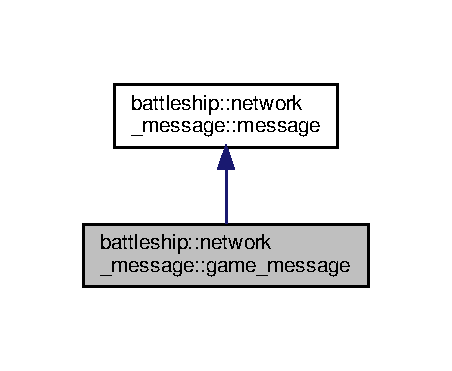
\includegraphics[width=217pt]{classbattleship_1_1network__message_1_1game__message__inherit__graph}
\end{center}
\end{figure}


Collaboration diagram for battleship\+:\+:network\+\_\+message\+:\+:game\+\_\+message\+:
\nopagebreak
\begin{figure}[H]
\begin{center}
\leavevmode
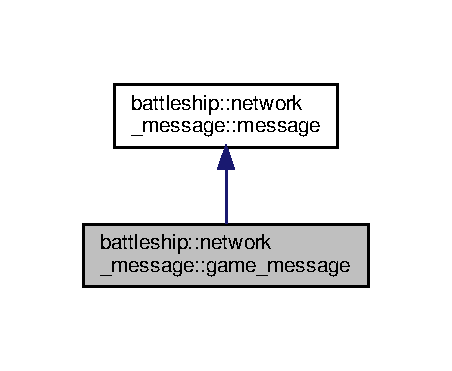
\includegraphics[width=217pt]{classbattleship_1_1network__message_1_1game__message__coll__graph}
\end{center}
\end{figure}
\subsection*{Public Member Functions}
\begin{DoxyCompactItemize}
\item 
virtual \hyperlink{classbattleship_1_1network__message_1_1game__message_ab3ceb7bc3b5fae4b4cf4ebd96fd6110f}{$\sim$game\+\_\+message} ()
\item 
const unsigned char \hyperlink{classbattleship_1_1network__message_1_1game__message_af64b2d72181dd2444616980c67d43581}{game\+\_\+id} () const
\end{DoxyCompactItemize}
\subsection*{Static Public Member Functions}
\begin{DoxyCompactItemize}
\item 
static \hyperlink{classbattleship_1_1network__message_1_1game__message}{game\+\_\+message} $\ast$ \hyperlink{classbattleship_1_1network__message_1_1game__message_a75f29d2d7fddfe52eb7755857a61aec6}{parse\+\_\+message} (const char $\ast$msg, const unsigned char len)
\item 
static \hyperlink{classbattleship_1_1network__message_1_1game__message}{game\+\_\+message} $\ast$ \hyperlink{classbattleship_1_1network__message_1_1game__message_aa1694088084ed2b07b6c06ba9fb2cb03}{create\+\_\+message} (const network\+\_\+message\+::signal msg\+\_\+signal, const unsigned char \hyperlink{classbattleship_1_1network__message_1_1message_af2ebed25f82de46c947a2241c6952563}{from}, const unsigned char \hyperlink{classbattleship_1_1network__message_1_1message_a36145cf7dfc9102da280adfad5d1a972}{to}, const unsigned char \hyperlink{classbattleship_1_1network__message_1_1game__message_af64b2d72181dd2444616980c67d43581}{game\+\_\+id}, const char $\ast$\hyperlink{classbattleship_1_1network__message_1_1message_ab42ddf52012135284f65641702459912}{payload}=nullptr, const unsigned char \hyperlink{classbattleship_1_1network__message_1_1message_ac4a236888d40ffbdd8572660a3f34b1e}{payload\+\_\+length}=0)
\end{DoxyCompactItemize}
\subsection*{Protected Member Functions}
\begin{DoxyCompactItemize}
\item 
\mbox{\Hypertarget{classbattleship_1_1network__message_1_1game__message_ae79588b4a84657987030ec8903b70338}\label{classbattleship_1_1network__message_1_1game__message_ae79588b4a84657987030ec8903b70338}} 
{\bfseries game\+\_\+message} (const char $\ast$msg, const unsigned char len)
\item 
\mbox{\Hypertarget{classbattleship_1_1network__message_1_1game__message_a6ec5d82b622c47f37ac0e81507eb7bdd}\label{classbattleship_1_1network__message_1_1game__message_a6ec5d82b622c47f37ac0e81507eb7bdd}} 
virtual unsigned char {\bfseries next\+\_\+available\+\_\+offset} () const
\end{DoxyCompactItemize}
\subsection*{Additional Inherited Members}


\subsection{Detailed Description}
Game network message class. 

\begin{DoxyAuthor}{Author}
Jonathan Henly 

Adham Kassem 
\end{DoxyAuthor}
\begin{DoxyVersion}{Version}
12-\/03-\/2018 
\end{DoxyVersion}


\subsection{Constructor \& Destructor Documentation}
\mbox{\Hypertarget{classbattleship_1_1network__message_1_1game__message_ab3ceb7bc3b5fae4b4cf4ebd96fd6110f}\label{classbattleship_1_1network__message_1_1game__message_ab3ceb7bc3b5fae4b4cf4ebd96fd6110f}} 
\index{battleship\+::network\+\_\+message\+::game\+\_\+message@{battleship\+::network\+\_\+message\+::game\+\_\+message}!````~game\+\_\+message@{$\sim$game\+\_\+message}}
\index{````~game\+\_\+message@{$\sim$game\+\_\+message}!battleship\+::network\+\_\+message\+::game\+\_\+message@{battleship\+::network\+\_\+message\+::game\+\_\+message}}
\subsubsection{\texorpdfstring{$\sim$game\+\_\+message()}{~game\_message()}}
{\footnotesize\ttfamily virtual battleship\+::network\+\_\+message\+::game\+\_\+message\+::$\sim$game\+\_\+message (\begin{DoxyParamCaption}{ }\end{DoxyParamCaption})\hspace{0.3cm}{\ttfamily [inline]}, {\ttfamily [virtual]}}

Calls
\begin{DoxyCode}
\textcolor{keyword}{virtual} \hyperlink{classbattleship_1_1network__message_1_1message_a89d002562fcc64e39f35782e92c4d6e2}{~message}() 
\end{DoxyCode}
 . 

\subsection{Member Function Documentation}
\mbox{\Hypertarget{classbattleship_1_1network__message_1_1game__message_aa1694088084ed2b07b6c06ba9fb2cb03}\label{classbattleship_1_1network__message_1_1game__message_aa1694088084ed2b07b6c06ba9fb2cb03}} 
\index{battleship\+::network\+\_\+message\+::game\+\_\+message@{battleship\+::network\+\_\+message\+::game\+\_\+message}!create\+\_\+message@{create\+\_\+message}}
\index{create\+\_\+message@{create\+\_\+message}!battleship\+::network\+\_\+message\+::game\+\_\+message@{battleship\+::network\+\_\+message\+::game\+\_\+message}}
\subsubsection{\texorpdfstring{create\+\_\+message()}{create\_message()}}
{\footnotesize\ttfamily static \hyperlink{classbattleship_1_1network__message_1_1game__message}{game\+\_\+message}$\ast$ battleship\+::network\+\_\+message\+::game\+\_\+message\+::create\+\_\+message (\begin{DoxyParamCaption}\item[{const network\+\_\+message\+::signal}]{msg\+\_\+signal,  }\item[{const unsigned char}]{from,  }\item[{const unsigned char}]{to,  }\item[{const unsigned char}]{game\+\_\+id,  }\item[{const char $\ast$}]{payload = {\ttfamily nullptr},  }\item[{const unsigned char}]{payload\+\_\+length = {\ttfamily 0} }\end{DoxyParamCaption})\hspace{0.3cm}{\ttfamily [inline]}, {\ttfamily [static]}}


\begin{DoxyParams}{Parameters}
{\em msg\+\_\+signal} & -\/ \\
\hline
{\em from} & -\/ \\
\hline
{\em to} & -\/ \\
\hline
{\em game\+\_\+id} & -\/ \\
\hline
{\em payload} & -\/ \\
\hline
{\em payload\+\_\+length} & -\/ \\
\hline
\end{DoxyParams}
\begin{DoxyReturn}{Returns}

\end{DoxyReturn}
\mbox{\Hypertarget{classbattleship_1_1network__message_1_1game__message_af64b2d72181dd2444616980c67d43581}\label{classbattleship_1_1network__message_1_1game__message_af64b2d72181dd2444616980c67d43581}} 
\index{battleship\+::network\+\_\+message\+::game\+\_\+message@{battleship\+::network\+\_\+message\+::game\+\_\+message}!game\+\_\+id@{game\+\_\+id}}
\index{game\+\_\+id@{game\+\_\+id}!battleship\+::network\+\_\+message\+::game\+\_\+message@{battleship\+::network\+\_\+message\+::game\+\_\+message}}
\subsubsection{\texorpdfstring{game\+\_\+id()}{game\_id()}}
{\footnotesize\ttfamily const unsigned char battleship\+::network\+\_\+message\+::game\+\_\+message\+::game\+\_\+id (\begin{DoxyParamCaption}{ }\end{DoxyParamCaption}) const\hspace{0.3cm}{\ttfamily [inline]}}

\begin{DoxyReturn}{Returns}
this message\textquotesingle{}s game ID. 
\end{DoxyReturn}
\mbox{\Hypertarget{classbattleship_1_1network__message_1_1game__message_a75f29d2d7fddfe52eb7755857a61aec6}\label{classbattleship_1_1network__message_1_1game__message_a75f29d2d7fddfe52eb7755857a61aec6}} 
\index{battleship\+::network\+\_\+message\+::game\+\_\+message@{battleship\+::network\+\_\+message\+::game\+\_\+message}!parse\+\_\+message@{parse\+\_\+message}}
\index{parse\+\_\+message@{parse\+\_\+message}!battleship\+::network\+\_\+message\+::game\+\_\+message@{battleship\+::network\+\_\+message\+::game\+\_\+message}}
\subsubsection{\texorpdfstring{parse\+\_\+message()}{parse\_message()}}
{\footnotesize\ttfamily static \hyperlink{classbattleship_1_1network__message_1_1game__message}{game\+\_\+message}$\ast$ battleship\+::network\+\_\+message\+::game\+\_\+message\+::parse\+\_\+message (\begin{DoxyParamCaption}\item[{const char $\ast$}]{msg,  }\item[{const unsigned char}]{len }\end{DoxyParamCaption})\hspace{0.3cm}{\ttfamily [inline]}, {\ttfamily [static]}}

Parses a message from a passed in \{ array\} of length
\begin{DoxyCode}
len 
\end{DoxyCode}
 .


\begin{DoxyParams}{Parameters}
{\em msg} & -\/ a correctly coded
\begin{DoxyCode}
\textcolor{keywordtype}{char} 
\end{DoxyCode}
 array. \\
\hline
{\em len} & -\/ the byte length of
\begin{DoxyCode}
msg 
\end{DoxyCode}
 .\\
\hline
\end{DoxyParams}
\begin{DoxyReturn}{Returns}
a smart pointer to a new message created from a passed in 
\begin{DoxyCode}
\textcolor{keywordtype}{char} 
\end{DoxyCode}
 array of length
\begin{DoxyCode}
len 
\end{DoxyCode}
 . 
\end{DoxyReturn}


The documentation for this class was generated from the following file\+:\begin{DoxyCompactItemize}
\item 
shared/inc/message.\+h\end{DoxyCompactItemize}

\hypertarget{classbattleship_1_1game__server_1_1game__pool}{}\section{battleship\+:\+:game\+\_\+server\+:\+:game\+\_\+pool Class Reference}
\label{classbattleship_1_1game__server_1_1game__pool}\index{battleship\+::game\+\_\+server\+::game\+\_\+pool@{battleship\+::game\+\_\+server\+::game\+\_\+pool}}


A thread safe game pool for holding server games.  




{\ttfamily \#include $<$gamepool.\+h$>$}

\subsection*{Public Member Functions}
\begin{DoxyCompactItemize}
\item 
\hyperlink{classbattleship_1_1game__server_1_1game__pool_a8f1683759e6491fe84b55409873c8163}{game\+\_\+pool} (const unsigned char max\+\_\+size)
\item 
\hyperlink{classbattleship_1_1game__server_1_1game__pool_a595c7d278fc0163b37780d90663663a2}{$\sim$game\+\_\+pool} ()
\item 
std\+::weak\+\_\+ptr$<$ \hyperlink{classbattleship_1_1game__server_1_1game}{game} $>$ \hyperlink{classbattleship_1_1game__server_1_1game__pool_a6d460991bba52fc0d04bd1ee65989ba2}{add\+\_\+ready\+\_\+client} (std\+::weak\+\_\+ptr$<$ \hyperlink{classbattleship_1_1game__server_1_1client}{client} $>$ r\+\_\+client)
\item 
bool \hyperlink{classbattleship_1_1game__server_1_1game__pool_a49cca84e56ae8a98559a6345d147511d}{remove} (const unsigned char game\+\_\+id)
\item 
const std\+::weak\+\_\+ptr$<$ \hyperlink{classbattleship_1_1game__server_1_1game}{game} $>$ \hyperlink{classbattleship_1_1game__server_1_1game__pool_ad6c1392c3842f1a37c762d1c27eba7d2}{get} (const unsigned char game\+\_\+id) const
\item 
std\+::unique\+\_\+lock$<$ std\+::mutex $>$ \hyperlink{classbattleship_1_1game__server_1_1game__pool_ae87384fc2dbf34f7f2769e8763c142b3}{get\+\_\+lock} ()
\item 
const std\+::shared\+\_\+ptr$<$ \hyperlink{classbattleship_1_1game__server_1_1game}{game} $>$ \hyperlink{classbattleship_1_1game__server_1_1game__pool_a47ebc8c0b2d4280ce0d02e0d808230e3}{get\+\_\+with\+\_\+lock} (std\+::unique\+\_\+lock$<$ std\+::mutex $>$ \&lock, const unsigned char game\+\_\+id)
\item 
unsigned char \hyperlink{classbattleship_1_1game__server_1_1game__pool_a4082a1a43dc489fae1d537126c7024c5}{get\+\_\+max\+\_\+game\+\_\+count} () const
\item 
unsigned char \hyperlink{classbattleship_1_1game__server_1_1game__pool_ae35839994dec4bd94fb1dc7134c1e1ff}{size} () const
\end{DoxyCompactItemize}


\subsection{Detailed Description}
A thread safe game pool for holding server games. 

\begin{DoxyAuthor}{Author}
Jonathan Henly 

Adham Kassem 
\end{DoxyAuthor}
\begin{DoxyVersion}{Version}
11-\/27-\/2018 
\end{DoxyVersion}


\subsection{Constructor \& Destructor Documentation}
\mbox{\Hypertarget{classbattleship_1_1game__server_1_1game__pool_a8f1683759e6491fe84b55409873c8163}\label{classbattleship_1_1game__server_1_1game__pool_a8f1683759e6491fe84b55409873c8163}} 
\index{battleship\+::game\+\_\+server\+::game\+\_\+pool@{battleship\+::game\+\_\+server\+::game\+\_\+pool}!game\+\_\+pool@{game\+\_\+pool}}
\index{game\+\_\+pool@{game\+\_\+pool}!battleship\+::game\+\_\+server\+::game\+\_\+pool@{battleship\+::game\+\_\+server\+::game\+\_\+pool}}
\subsubsection{\texorpdfstring{game\+\_\+pool()}{game\_pool()}}
{\footnotesize\ttfamily battleship\+::game\+\_\+server\+::game\+\_\+pool\+::game\+\_\+pool (\begin{DoxyParamCaption}\item[{const unsigned char}]{max\+\_\+size }\end{DoxyParamCaption})\hspace{0.3cm}{\ttfamily [explicit]}}

Creates a client pool with a maximum number of allowed clients.


\begin{DoxyParams}{Parameters}
{\em max\+\_\+size} & -\/ the maximum number of clients allowed in this pool. \\
\hline
\end{DoxyParams}
\mbox{\Hypertarget{classbattleship_1_1game__server_1_1game__pool_a595c7d278fc0163b37780d90663663a2}\label{classbattleship_1_1game__server_1_1game__pool_a595c7d278fc0163b37780d90663663a2}} 
\index{battleship\+::game\+\_\+server\+::game\+\_\+pool@{battleship\+::game\+\_\+server\+::game\+\_\+pool}!````~game\+\_\+pool@{$\sim$game\+\_\+pool}}
\index{````~game\+\_\+pool@{$\sim$game\+\_\+pool}!battleship\+::game\+\_\+server\+::game\+\_\+pool@{battleship\+::game\+\_\+server\+::game\+\_\+pool}}
\subsubsection{\texorpdfstring{$\sim$game\+\_\+pool()}{~game\_pool()}}
{\footnotesize\ttfamily battleship\+::game\+\_\+server\+::game\+\_\+pool\+::$\sim$game\+\_\+pool (\begin{DoxyParamCaption}{ }\end{DoxyParamCaption})\hspace{0.3cm}{\ttfamily [inline]}}

Default destructor. 

\subsection{Member Function Documentation}
\mbox{\Hypertarget{classbattleship_1_1game__server_1_1game__pool_a6d460991bba52fc0d04bd1ee65989ba2}\label{classbattleship_1_1game__server_1_1game__pool_a6d460991bba52fc0d04bd1ee65989ba2}} 
\index{battleship\+::game\+\_\+server\+::game\+\_\+pool@{battleship\+::game\+\_\+server\+::game\+\_\+pool}!add\+\_\+ready\+\_\+client@{add\+\_\+ready\+\_\+client}}
\index{add\+\_\+ready\+\_\+client@{add\+\_\+ready\+\_\+client}!battleship\+::game\+\_\+server\+::game\+\_\+pool@{battleship\+::game\+\_\+server\+::game\+\_\+pool}}
\subsubsection{\texorpdfstring{add\+\_\+ready\+\_\+client()}{add\_ready\_client()}}
{\footnotesize\ttfamily std\+::weak\+\_\+ptr$<$ \hyperlink{classbattleship_1_1game__server_1_1game}{game} $>$ battleship\+::game\+\_\+server\+::game\+\_\+pool\+::add\+\_\+ready\+\_\+client (\begin{DoxyParamCaption}\item[{std\+::weak\+\_\+ptr$<$ \hyperlink{classbattleship_1_1game__server_1_1client}{client} $>$}]{r\+\_\+client }\end{DoxyParamCaption})}


\begin{DoxyParams}{Parameters}
{\em client\+\_\+id} & \\
\hline
\end{DoxyParams}
\begin{DoxyReturn}{Returns}

\end{DoxyReturn}
\mbox{\Hypertarget{classbattleship_1_1game__server_1_1game__pool_ad6c1392c3842f1a37c762d1c27eba7d2}\label{classbattleship_1_1game__server_1_1game__pool_ad6c1392c3842f1a37c762d1c27eba7d2}} 
\index{battleship\+::game\+\_\+server\+::game\+\_\+pool@{battleship\+::game\+\_\+server\+::game\+\_\+pool}!get@{get}}
\index{get@{get}!battleship\+::game\+\_\+server\+::game\+\_\+pool@{battleship\+::game\+\_\+server\+::game\+\_\+pool}}
\subsubsection{\texorpdfstring{get()}{get()}}
{\footnotesize\ttfamily const std\+::weak\+\_\+ptr$<$ \hyperlink{classbattleship_1_1game__server_1_1game}{game} $>$ battleship\+::game\+\_\+server\+::game\+\_\+pool\+::get (\begin{DoxyParamCaption}\item[{const unsigned char}]{game\+\_\+id }\end{DoxyParamCaption}) const}

Gets the game, whose ID matches the passed in ID, from this game pool instance.

This method is the reader version of
\begin{DoxyCode}
\hyperlink{classbattleship_1_1game__server_1_1game__pool_a47ebc8c0b2d4280ce0d02e0d808230e3}{game\_pool::get\_with\_lock} 
\end{DoxyCode}
 .

Note\+: this method will return an empty
\begin{DoxyCode}
std::weak\_ptr<game> 
\end{DoxyCode}
 if the specified game ID is not found in this game pool.


\begin{DoxyParams}{Parameters}
{\em game\+\_\+id} & -\/ the ID of the game to retrieve. \\
\hline
\end{DoxyParams}
\begin{DoxyReturn}{Returns}
the game whose ID is
\begin{DoxyCode}
game\_id 
\end{DoxyCode}
 or
\begin{DoxyCode}
\textcolor{keyword}{nullptr} 
\end{DoxyCode}
 . 
\end{DoxyReturn}
\mbox{\Hypertarget{classbattleship_1_1game__server_1_1game__pool_ae87384fc2dbf34f7f2769e8763c142b3}\label{classbattleship_1_1game__server_1_1game__pool_ae87384fc2dbf34f7f2769e8763c142b3}} 
\index{battleship\+::game\+\_\+server\+::game\+\_\+pool@{battleship\+::game\+\_\+server\+::game\+\_\+pool}!get\+\_\+lock@{get\+\_\+lock}}
\index{get\+\_\+lock@{get\+\_\+lock}!battleship\+::game\+\_\+server\+::game\+\_\+pool@{battleship\+::game\+\_\+server\+::game\+\_\+pool}}
\subsubsection{\texorpdfstring{get\+\_\+lock()}{get\_lock()}}
{\footnotesize\ttfamily std\+::unique\+\_\+lock$<$ std\+::mutex $>$ battleship\+::game\+\_\+server\+::game\+\_\+pool\+::get\+\_\+lock (\begin{DoxyParamCaption}{ }\end{DoxyParamCaption})}

Acquires and returns a lock on this pool\textquotesingle{}s mutex. This method blocks until the lock can be acquired.

Note\+: if not manually released, the returned lock will release once the calling site goes out of scope.

\begin{DoxyReturn}{Returns}
a lock on this client pool\textquotesingle{}s mutex.
\end{DoxyReturn}
\begin{DoxySeeAlso}{See also}
\hyperlink{classbattleship_1_1game__server_1_1game__pool_a47ebc8c0b2d4280ce0d02e0d808230e3}{game\+\_\+pool\+::get\+\_\+with\+\_\+lock} 
\end{DoxySeeAlso}
\mbox{\Hypertarget{classbattleship_1_1game__server_1_1game__pool_a4082a1a43dc489fae1d537126c7024c5}\label{classbattleship_1_1game__server_1_1game__pool_a4082a1a43dc489fae1d537126c7024c5}} 
\index{battleship\+::game\+\_\+server\+::game\+\_\+pool@{battleship\+::game\+\_\+server\+::game\+\_\+pool}!get\+\_\+max\+\_\+game\+\_\+count@{get\+\_\+max\+\_\+game\+\_\+count}}
\index{get\+\_\+max\+\_\+game\+\_\+count@{get\+\_\+max\+\_\+game\+\_\+count}!battleship\+::game\+\_\+server\+::game\+\_\+pool@{battleship\+::game\+\_\+server\+::game\+\_\+pool}}
\subsubsection{\texorpdfstring{get\+\_\+max\+\_\+game\+\_\+count()}{get\_max\_game\_count()}}
{\footnotesize\ttfamily unsigned char battleship\+::game\+\_\+server\+::game\+\_\+pool\+::get\+\_\+max\+\_\+game\+\_\+count (\begin{DoxyParamCaption}{ }\end{DoxyParamCaption}) const\hspace{0.3cm}{\ttfamily [inline]}}

Gets the maximum number of games allowed in this pool instance. \begin{DoxyReturn}{Returns}
the max number of games allowed in this pool. 
\end{DoxyReturn}
\mbox{\Hypertarget{classbattleship_1_1game__server_1_1game__pool_a47ebc8c0b2d4280ce0d02e0d808230e3}\label{classbattleship_1_1game__server_1_1game__pool_a47ebc8c0b2d4280ce0d02e0d808230e3}} 
\index{battleship\+::game\+\_\+server\+::game\+\_\+pool@{battleship\+::game\+\_\+server\+::game\+\_\+pool}!get\+\_\+with\+\_\+lock@{get\+\_\+with\+\_\+lock}}
\index{get\+\_\+with\+\_\+lock@{get\+\_\+with\+\_\+lock}!battleship\+::game\+\_\+server\+::game\+\_\+pool@{battleship\+::game\+\_\+server\+::game\+\_\+pool}}
\subsubsection{\texorpdfstring{get\+\_\+with\+\_\+lock()}{get\_with\_lock()}}
{\footnotesize\ttfamily const std\+::shared\+\_\+ptr$<$ \hyperlink{classbattleship_1_1game__server_1_1game}{game} $>$ battleship\+::game\+\_\+server\+::game\+\_\+pool\+::get\+\_\+with\+\_\+lock (\begin{DoxyParamCaption}\item[{std\+::unique\+\_\+lock$<$ std\+::mutex $>$ \&}]{lock,  }\item[{const unsigned char}]{game\+\_\+id }\end{DoxyParamCaption})}

Gets the client with specified client ID, from this client pool instance, while owning this pool\textquotesingle{}s writer mutex lock.

This method is the writer version of
\begin{DoxyCode}
\hyperlink{classbattleship_1_1game__server_1_1game__pool_ad6c1392c3842f1a37c762d1c27eba7d2}{game\_pool::get} 
\end{DoxyCode}
 . It is used in conjunction with
\begin{DoxyCode}
\hyperlink{classbattleship_1_1game__server_1_1game__pool_ae87384fc2dbf34f7f2769e8763c142b3}{game\_pool::get\_lock} 
\end{DoxyCode}
 to safely update the state of a client.

Note\+: this method will return
\begin{DoxyCode}
\textcolor{keyword}{nullptr} 
\end{DoxyCode}
 if the specified client ID is not found in this client pool.


\begin{DoxyParams}{Parameters}
{\em lock} & -\/ the writer lock obtained from
\begin{DoxyCode}
\hyperlink{classbattleship_1_1game__server_1_1game__pool_ae87384fc2dbf34f7f2769e8763c142b3}{game\_pool::get\_lock} 
\end{DoxyCode}
 . \\
\hline
{\em client\+Id} & -\/ the ID of the client to get.\\
\hline
\end{DoxyParams}
\begin{DoxyReturn}{Returns}
a safe pointer with the client matching the specified client ID, or 
\begin{DoxyCode}
\textcolor{keyword}{nullptr} 
\end{DoxyCode}
 .
\end{DoxyReturn}
\begin{DoxySeeAlso}{See also}
\hyperlink{classbattleship_1_1game__server_1_1game__pool_ae87384fc2dbf34f7f2769e8763c142b3}{game\+\_\+pool\+::get\+\_\+lock} 

\hyperlink{classbattleship_1_1game__server_1_1game__pool_ad6c1392c3842f1a37c762d1c27eba7d2}{game\+\_\+pool\+::get} 
\end{DoxySeeAlso}
\mbox{\Hypertarget{classbattleship_1_1game__server_1_1game__pool_a49cca84e56ae8a98559a6345d147511d}\label{classbattleship_1_1game__server_1_1game__pool_a49cca84e56ae8a98559a6345d147511d}} 
\index{battleship\+::game\+\_\+server\+::game\+\_\+pool@{battleship\+::game\+\_\+server\+::game\+\_\+pool}!remove@{remove}}
\index{remove@{remove}!battleship\+::game\+\_\+server\+::game\+\_\+pool@{battleship\+::game\+\_\+server\+::game\+\_\+pool}}
\subsubsection{\texorpdfstring{remove()}{remove()}}
{\footnotesize\ttfamily bool battleship\+::game\+\_\+server\+::game\+\_\+pool\+::remove (\begin{DoxyParamCaption}\item[{const unsigned char}]{game\+\_\+id }\end{DoxyParamCaption})}

To\+Do finish documentation

Finally, it makes the specified client ID available for re-\/use and decreases the game count by one.


\begin{DoxyParams}{Parameters}
{\em game\+Id} & -\/ the ID of the game to remove. \\
\hline
\end{DoxyParams}
\begin{DoxyReturn}{Returns}
true if the game with matching specified ID was removed from this pool, otherwise false. 
\end{DoxyReturn}
\mbox{\Hypertarget{classbattleship_1_1game__server_1_1game__pool_ae35839994dec4bd94fb1dc7134c1e1ff}\label{classbattleship_1_1game__server_1_1game__pool_ae35839994dec4bd94fb1dc7134c1e1ff}} 
\index{battleship\+::game\+\_\+server\+::game\+\_\+pool@{battleship\+::game\+\_\+server\+::game\+\_\+pool}!size@{size}}
\index{size@{size}!battleship\+::game\+\_\+server\+::game\+\_\+pool@{battleship\+::game\+\_\+server\+::game\+\_\+pool}}
\subsubsection{\texorpdfstring{size()}{size()}}
{\footnotesize\ttfamily unsigned char battleship\+::game\+\_\+server\+::game\+\_\+pool\+::size (\begin{DoxyParamCaption}{ }\end{DoxyParamCaption}) const\hspace{0.3cm}{\ttfamily [inline]}}

Gets the number of games in this pool. \begin{DoxyReturn}{Returns}
the number of games in this pool. 
\end{DoxyReturn}


The documentation for this class was generated from the following files\+:\begin{DoxyCompactItemize}
\item 
inc/gamepool.\+h\item 
src/gamepool.\+cpp\end{DoxyCompactItemize}

\hypertarget{classbattleship_1_1network__message_1_1message}{}\section{battleship\+:\+:network\+\_\+message\+:\+:message Class Reference}
\label{classbattleship_1_1network__message_1_1message}\index{battleship\+::network\+\_\+message\+::message@{battleship\+::network\+\_\+message\+::message}}


Base network messaging class.  




{\ttfamily \#include $<$message.\+h$>$}



Inheritance diagram for battleship\+:\+:network\+\_\+message\+:\+:message\+:
\nopagebreak
\begin{figure}[H]
\begin{center}
\leavevmode
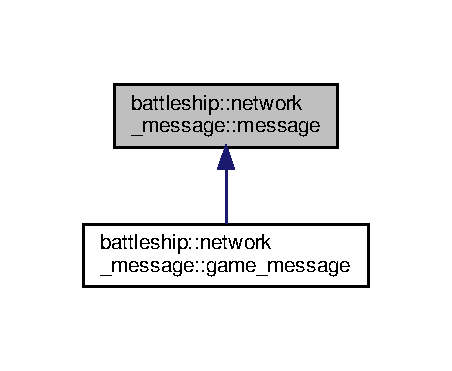
\includegraphics[width=217pt]{classbattleship_1_1network__message_1_1message__inherit__graph}
\end{center}
\end{figure}
\subsection*{Public Member Functions}
\begin{DoxyCompactItemize}
\item 
virtual \hyperlink{classbattleship_1_1network__message_1_1message_a89d002562fcc64e39f35782e92c4d6e2}{$\sim$message} ()
\item 
const char $\ast$ \hyperlink{classbattleship_1_1network__message_1_1message_aa0c2c52cb41c9c524e9e785a8240c60c}{msg} () const
\item 
const size\+\_\+t \hyperlink{classbattleship_1_1network__message_1_1message_a522b961254d0359c6c68bd32875a5626}{length} () const
\item 
const network\+\_\+message\+::type \hyperlink{classbattleship_1_1network__message_1_1message_a19cd4318b0e70831ddbf340597d040a4}{type} () const
\item 
const network\+\_\+message\+::signal \hyperlink{classbattleship_1_1network__message_1_1message_a5709b3059dfb73e135dca1c6f248f797}{signal} () const
\item 
const unsigned char \hyperlink{classbattleship_1_1network__message_1_1message_af2ebed25f82de46c947a2241c6952563}{from} () const
\item 
const unsigned char \hyperlink{classbattleship_1_1network__message_1_1message_a36145cf7dfc9102da280adfad5d1a972}{to} () const
\item 
const bool \hyperlink{classbattleship_1_1network__message_1_1message_a2232a3db5d5244e5487968908c04b9f9}{has\+\_\+payload} () const
\item 
const char $\ast$ \hyperlink{classbattleship_1_1network__message_1_1message_ab42ddf52012135284f65641702459912}{payload} () const
\item 
const unsigned char \hyperlink{classbattleship_1_1network__message_1_1message_ac4a236888d40ffbdd8572660a3f34b1e}{payload\+\_\+length} () const
\end{DoxyCompactItemize}
\subsection*{Static Public Member Functions}
\begin{DoxyCompactItemize}
\item 
static \hyperlink{classbattleship_1_1network__message_1_1message}{message} $\ast$ \hyperlink{classbattleship_1_1network__message_1_1message_a8f87e24d9328257a0f76278a0802f86c}{parse\+\_\+message} (const char $\ast$msg, const unsigned char len)
\item 
static \hyperlink{classbattleship_1_1network__message_1_1message}{message} $\ast$ \hyperlink{classbattleship_1_1network__message_1_1message_aa50f58d9553f3532071c9acda7b1f031}{create\+\_\+message} (const network\+\_\+message\+::type m\+\_\+type, const network\+\_\+message\+::signal m\+\_\+signal, const unsigned char \hyperlink{classbattleship_1_1network__message_1_1message_af2ebed25f82de46c947a2241c6952563}{from}, const unsigned char \hyperlink{classbattleship_1_1network__message_1_1message_a36145cf7dfc9102da280adfad5d1a972}{to}, const char $\ast$\hyperlink{classbattleship_1_1network__message_1_1message_ab42ddf52012135284f65641702459912}{payload}=nullptr, const unsigned char \hyperlink{classbattleship_1_1network__message_1_1message_ac4a236888d40ffbdd8572660a3f34b1e}{payload\+\_\+length}=0)
\item 
static \hyperlink{classbattleship_1_1network__message_1_1message}{message} $\ast$ \hyperlink{classbattleship_1_1network__message_1_1message_aa55c4377f51cfd59e1d0c6abd4295d4f}{create\+\_\+message} (const network\+\_\+message\+::type m\+\_\+type, const network\+\_\+message\+::signal m\+\_\+signal, const unsigned char \hyperlink{classbattleship_1_1network__message_1_1message_af2ebed25f82de46c947a2241c6952563}{from}, const unsigned char \hyperlink{classbattleship_1_1network__message_1_1message_a36145cf7dfc9102da280adfad5d1a972}{to}, const std\+::string \hyperlink{classbattleship_1_1network__message_1_1message_ab42ddf52012135284f65641702459912}{payload})
\end{DoxyCompactItemize}
\subsection*{Protected Member Functions}
\begin{DoxyCompactItemize}
\item 
\mbox{\Hypertarget{classbattleship_1_1network__message_1_1message_a8648ab9741e0a2617e79a2a33b816597}\label{classbattleship_1_1network__message_1_1message_a8648ab9741e0a2617e79a2a33b816597}} 
{\bfseries message} (const char $\ast$msg, const unsigned char len)
\item 
\mbox{\Hypertarget{classbattleship_1_1network__message_1_1message_a4cc5125a5a6f24e1bc31db2b9457d0f9}\label{classbattleship_1_1network__message_1_1message_a4cc5125a5a6f24e1bc31db2b9457d0f9}} 
{\bfseries message} (const network\+\_\+message\+::type m\+\_\+type, const network\+\_\+message\+::signal m\+\_\+signal, const unsigned char \hyperlink{classbattleship_1_1network__message_1_1message_af2ebed25f82de46c947a2241c6952563}{from}, const unsigned char \hyperlink{classbattleship_1_1network__message_1_1message_a36145cf7dfc9102da280adfad5d1a972}{to}, const char $\ast$\hyperlink{classbattleship_1_1network__message_1_1message_ab42ddf52012135284f65641702459912}{payload}=nullptr, const unsigned char \hyperlink{classbattleship_1_1network__message_1_1message_ac4a236888d40ffbdd8572660a3f34b1e}{payload\+\_\+length}=0)
\item 
\mbox{\Hypertarget{classbattleship_1_1network__message_1_1message_a8e025f494428c0e498341dcac119155e}\label{classbattleship_1_1network__message_1_1message_a8e025f494428c0e498341dcac119155e}} 
const char {\bfseries message\+\_\+terminator} ()
\item 
\mbox{\Hypertarget{classbattleship_1_1network__message_1_1message_ac410b96d54dffc60f16c459b7d4ecc94}\label{classbattleship_1_1network__message_1_1message_ac410b96d54dffc60f16c459b7d4ecc94}} 
virtual unsigned char {\bfseries next\+\_\+available\+\_\+offset} () const
\item 
\mbox{\Hypertarget{classbattleship_1_1network__message_1_1message_a390532050b2c6e513a3b3aa666878f37}\label{classbattleship_1_1network__message_1_1message_a390532050b2c6e513a3b3aa666878f37}} 
char $\ast$ {\bfseries msg} ()
\end{DoxyCompactItemize}
\subsection*{Static Protected Attributes}
\begin{DoxyCompactItemize}
\item 
\mbox{\Hypertarget{classbattleship_1_1network__message_1_1message_af14888193de7e2a1fc8309301ae903bd}\label{classbattleship_1_1network__message_1_1message_af14888193de7e2a1fc8309301ae903bd}} 
static const unsigned char {\bfseries T\+Y\+P\+E\+\_\+\+O\+F\+F\+S\+ET} = 0
\item 
\mbox{\Hypertarget{classbattleship_1_1network__message_1_1message_a3b8b9ed0e5af5e4af3182d4380d7e13f}\label{classbattleship_1_1network__message_1_1message_a3b8b9ed0e5af5e4af3182d4380d7e13f}} 
static const unsigned char {\bfseries S\+I\+G\+N\+A\+L\+\_\+\+O\+F\+F\+S\+ET} = 1
\item 
\mbox{\Hypertarget{classbattleship_1_1network__message_1_1message_ac5e61619d74437ba3debfd7eac03b1d6}\label{classbattleship_1_1network__message_1_1message_ac5e61619d74437ba3debfd7eac03b1d6}} 
static const unsigned char {\bfseries F\+R\+O\+M\+\_\+\+O\+F\+F\+S\+ET} = 2
\item 
\mbox{\Hypertarget{classbattleship_1_1network__message_1_1message_a692694320d13692d056e7c859758d38f}\label{classbattleship_1_1network__message_1_1message_a692694320d13692d056e7c859758d38f}} 
static const unsigned char {\bfseries T\+O\+\_\+\+O\+F\+F\+S\+ET} = 3
\item 
\mbox{\Hypertarget{classbattleship_1_1network__message_1_1message_aa44f97189eacff487d14b54b469e40d7}\label{classbattleship_1_1network__message_1_1message_aa44f97189eacff487d14b54b469e40d7}} 
static const unsigned char {\bfseries H\+A\+S\+\_\+\+P\+A\+Y\+L\+O\+A\+D\+\_\+\+O\+F\+F\+S\+ET} = 4
\item 
\mbox{\Hypertarget{classbattleship_1_1network__message_1_1message_adbbec67faaa06ff9bbb8defbff091f44}\label{classbattleship_1_1network__message_1_1message_adbbec67faaa06ff9bbb8defbff091f44}} 
static const unsigned char {\bfseries P\+A\+Y\+L\+O\+A\+D\+\_\+\+O\+F\+F\+S\+ET} = 5
\end{DoxyCompactItemize}


\subsection{Detailed Description}
Base network messaging class. 

\begin{DoxyAuthor}{Author}
Jonathan Henly 

Adham Kassem 
\end{DoxyAuthor}
\begin{DoxyVersion}{Version}
12-\/03-\/2018 
\end{DoxyVersion}


\subsection{Constructor \& Destructor Documentation}
\mbox{\Hypertarget{classbattleship_1_1network__message_1_1message_a89d002562fcc64e39f35782e92c4d6e2}\label{classbattleship_1_1network__message_1_1message_a89d002562fcc64e39f35782e92c4d6e2}} 
\index{battleship\+::network\+\_\+message\+::message@{battleship\+::network\+\_\+message\+::message}!````~message@{$\sim$message}}
\index{````~message@{$\sim$message}!battleship\+::network\+\_\+message\+::message@{battleship\+::network\+\_\+message\+::message}}
\subsubsection{\texorpdfstring{$\sim$message()}{~message()}}
{\footnotesize\ttfamily virtual battleship\+::network\+\_\+message\+::message\+::$\sim$message (\begin{DoxyParamCaption}{ }\end{DoxyParamCaption})\hspace{0.3cm}{\ttfamily [inline]}, {\ttfamily [virtual]}}

Deletes this message\textquotesingle{}s underlying
\begin{DoxyCode}
\textcolor{keywordtype}{char} 
\end{DoxyCode}
 array. 

\subsection{Member Function Documentation}
\mbox{\Hypertarget{classbattleship_1_1network__message_1_1message_aa50f58d9553f3532071c9acda7b1f031}\label{classbattleship_1_1network__message_1_1message_aa50f58d9553f3532071c9acda7b1f031}} 
\index{battleship\+::network\+\_\+message\+::message@{battleship\+::network\+\_\+message\+::message}!create\+\_\+message@{create\+\_\+message}}
\index{create\+\_\+message@{create\+\_\+message}!battleship\+::network\+\_\+message\+::message@{battleship\+::network\+\_\+message\+::message}}
\subsubsection{\texorpdfstring{create\+\_\+message()}{create\_message()}\hspace{0.1cm}{\footnotesize\ttfamily [1/2]}}
{\footnotesize\ttfamily static \hyperlink{classbattleship_1_1network__message_1_1message}{message}$\ast$ battleship\+::network\+\_\+message\+::message\+::create\+\_\+message (\begin{DoxyParamCaption}\item[{const network\+\_\+message\+::type}]{m\+\_\+type,  }\item[{const network\+\_\+message\+::signal}]{m\+\_\+signal,  }\item[{const unsigned char}]{from,  }\item[{const unsigned char}]{to,  }\item[{const char $\ast$}]{payload = {\ttfamily nullptr},  }\item[{const unsigned char}]{payload\+\_\+length = {\ttfamily 0} }\end{DoxyParamCaption})\hspace{0.3cm}{\ttfamily [inline]}, {\ttfamily [static]}}

Create a message from the specified arguments.


\begin{DoxyParams}{Parameters}
{\em m\+\_\+type} & -\/ the type of message. \\
\hline
{\em m\+\_\+signal} & -\/ what the message signals. \\
\hline
{\em from} & -\/ the ID of the sender. \\
\hline
{\em to} & -\/ the ID of the recipient. \\
\hline
{\em payload} & -\/ this message\textquotesingle{}s optional payload. \\
\hline
{\em payload\+\_\+length} & -\/ length of optional payload.\\
\hline
\end{DoxyParams}
\begin{DoxyReturn}{Returns}
a smart pointer holding this newly created message. 
\end{DoxyReturn}
\mbox{\Hypertarget{classbattleship_1_1network__message_1_1message_aa55c4377f51cfd59e1d0c6abd4295d4f}\label{classbattleship_1_1network__message_1_1message_aa55c4377f51cfd59e1d0c6abd4295d4f}} 
\index{battleship\+::network\+\_\+message\+::message@{battleship\+::network\+\_\+message\+::message}!create\+\_\+message@{create\+\_\+message}}
\index{create\+\_\+message@{create\+\_\+message}!battleship\+::network\+\_\+message\+::message@{battleship\+::network\+\_\+message\+::message}}
\subsubsection{\texorpdfstring{create\+\_\+message()}{create\_message()}\hspace{0.1cm}{\footnotesize\ttfamily [2/2]}}
{\footnotesize\ttfamily static \hyperlink{classbattleship_1_1network__message_1_1message}{message}$\ast$ battleship\+::network\+\_\+message\+::message\+::create\+\_\+message (\begin{DoxyParamCaption}\item[{const network\+\_\+message\+::type}]{m\+\_\+type,  }\item[{const network\+\_\+message\+::signal}]{m\+\_\+signal,  }\item[{const unsigned char}]{from,  }\item[{const unsigned char}]{to,  }\item[{const std\+::string}]{payload }\end{DoxyParamCaption})\hspace{0.3cm}{\ttfamily [inline]}, {\ttfamily [static]}}

Create a message from the specified arguments.


\begin{DoxyParams}{Parameters}
{\em m\+\_\+type} & -\/ the type of message. \\
\hline
{\em m\+\_\+signal} & -\/ what the message signals. \\
\hline
{\em from} & -\/ the ID of the sender. \\
\hline
{\em to} & -\/ the ID of the recipient. \\
\hline
{\em payload} & -\/ the body of this messsage.\\
\hline
\end{DoxyParams}
\begin{DoxyReturn}{Returns}
a smart pointer holding this newly created message. 
\end{DoxyReturn}
\mbox{\Hypertarget{classbattleship_1_1network__message_1_1message_af2ebed25f82de46c947a2241c6952563}\label{classbattleship_1_1network__message_1_1message_af2ebed25f82de46c947a2241c6952563}} 
\index{battleship\+::network\+\_\+message\+::message@{battleship\+::network\+\_\+message\+::message}!from@{from}}
\index{from@{from}!battleship\+::network\+\_\+message\+::message@{battleship\+::network\+\_\+message\+::message}}
\subsubsection{\texorpdfstring{from()}{from()}}
{\footnotesize\ttfamily const unsigned char battleship\+::network\+\_\+message\+::message\+::from (\begin{DoxyParamCaption}{ }\end{DoxyParamCaption}) const\hspace{0.3cm}{\ttfamily [inline]}}

\begin{DoxyReturn}{Returns}
the sender ID of this message. 
\end{DoxyReturn}
\mbox{\Hypertarget{classbattleship_1_1network__message_1_1message_a2232a3db5d5244e5487968908c04b9f9}\label{classbattleship_1_1network__message_1_1message_a2232a3db5d5244e5487968908c04b9f9}} 
\index{battleship\+::network\+\_\+message\+::message@{battleship\+::network\+\_\+message\+::message}!has\+\_\+payload@{has\+\_\+payload}}
\index{has\+\_\+payload@{has\+\_\+payload}!battleship\+::network\+\_\+message\+::message@{battleship\+::network\+\_\+message\+::message}}
\subsubsection{\texorpdfstring{has\+\_\+payload()}{has\_payload()}}
{\footnotesize\ttfamily const bool battleship\+::network\+\_\+message\+::message\+::has\+\_\+payload (\begin{DoxyParamCaption}{ }\end{DoxyParamCaption}) const\hspace{0.3cm}{\ttfamily [inline]}}

\begin{DoxyReturn}{Returns}
true if this message has a payload, otherwise false. 
\end{DoxyReturn}
\mbox{\Hypertarget{classbattleship_1_1network__message_1_1message_a522b961254d0359c6c68bd32875a5626}\label{classbattleship_1_1network__message_1_1message_a522b961254d0359c6c68bd32875a5626}} 
\index{battleship\+::network\+\_\+message\+::message@{battleship\+::network\+\_\+message\+::message}!length@{length}}
\index{length@{length}!battleship\+::network\+\_\+message\+::message@{battleship\+::network\+\_\+message\+::message}}
\subsubsection{\texorpdfstring{length()}{length()}}
{\footnotesize\ttfamily const size\+\_\+t battleship\+::network\+\_\+message\+::message\+::length (\begin{DoxyParamCaption}{ }\end{DoxyParamCaption}) const\hspace{0.3cm}{\ttfamily [inline]}}

\begin{DoxyReturn}{Returns}
the length of this message. 
\end{DoxyReturn}
\mbox{\Hypertarget{classbattleship_1_1network__message_1_1message_aa0c2c52cb41c9c524e9e785a8240c60c}\label{classbattleship_1_1network__message_1_1message_aa0c2c52cb41c9c524e9e785a8240c60c}} 
\index{battleship\+::network\+\_\+message\+::message@{battleship\+::network\+\_\+message\+::message}!msg@{msg}}
\index{msg@{msg}!battleship\+::network\+\_\+message\+::message@{battleship\+::network\+\_\+message\+::message}}
\subsubsection{\texorpdfstring{msg()}{msg()}}
{\footnotesize\ttfamily const char$\ast$ battleship\+::network\+\_\+message\+::message\+::msg (\begin{DoxyParamCaption}{ }\end{DoxyParamCaption}) const\hspace{0.3cm}{\ttfamily [inline]}}

\begin{DoxyReturn}{Returns}
the underlying message
\begin{DoxyCode}
\textcolor{keywordtype}{char} 
\end{DoxyCode}
 array. 
\end{DoxyReturn}
\mbox{\Hypertarget{classbattleship_1_1network__message_1_1message_a8f87e24d9328257a0f76278a0802f86c}\label{classbattleship_1_1network__message_1_1message_a8f87e24d9328257a0f76278a0802f86c}} 
\index{battleship\+::network\+\_\+message\+::message@{battleship\+::network\+\_\+message\+::message}!parse\+\_\+message@{parse\+\_\+message}}
\index{parse\+\_\+message@{parse\+\_\+message}!battleship\+::network\+\_\+message\+::message@{battleship\+::network\+\_\+message\+::message}}
\subsubsection{\texorpdfstring{parse\+\_\+message()}{parse\_message()}}
{\footnotesize\ttfamily static \hyperlink{classbattleship_1_1network__message_1_1message}{message}$\ast$ battleship\+::network\+\_\+message\+::message\+::parse\+\_\+message (\begin{DoxyParamCaption}\item[{const char $\ast$}]{msg,  }\item[{const unsigned char}]{len }\end{DoxyParamCaption})\hspace{0.3cm}{\ttfamily [inline]}, {\ttfamily [static]}}

Parses a message from a passed in
\begin{DoxyCode}
\textcolor{keywordtype}{char} 
\end{DoxyCode}
 array of length 
\begin{DoxyCode}
len 
\end{DoxyCode}
 .


\begin{DoxyParams}{Parameters}
{\em msg} & -\/ a correctly coded
\begin{DoxyCode}
\textcolor{keywordtype}{char} 
\end{DoxyCode}
 array. \\
\hline
{\em len} & -\/ the byte length of
\begin{DoxyCode}
msg 
\end{DoxyCode}
 .\\
\hline
\end{DoxyParams}
\begin{DoxyReturn}{Returns}
a smart pointer holding a newly created message from a passed in 
\begin{DoxyCode}
\textcolor{keywordtype}{char} 
\end{DoxyCode}
 array of length
\begin{DoxyCode}
len 
\end{DoxyCode}
 . 
\end{DoxyReturn}
\mbox{\Hypertarget{classbattleship_1_1network__message_1_1message_ab42ddf52012135284f65641702459912}\label{classbattleship_1_1network__message_1_1message_ab42ddf52012135284f65641702459912}} 
\index{battleship\+::network\+\_\+message\+::message@{battleship\+::network\+\_\+message\+::message}!payload@{payload}}
\index{payload@{payload}!battleship\+::network\+\_\+message\+::message@{battleship\+::network\+\_\+message\+::message}}
\subsubsection{\texorpdfstring{payload()}{payload()}}
{\footnotesize\ttfamily const char$\ast$ battleship\+::network\+\_\+message\+::message\+::payload (\begin{DoxyParamCaption}{ }\end{DoxyParamCaption}) const\hspace{0.3cm}{\ttfamily [inline]}}

\begin{DoxyReturn}{Returns}
a pointer to this message\textquotesingle{}s payload. 
\end{DoxyReturn}
\mbox{\Hypertarget{classbattleship_1_1network__message_1_1message_ac4a236888d40ffbdd8572660a3f34b1e}\label{classbattleship_1_1network__message_1_1message_ac4a236888d40ffbdd8572660a3f34b1e}} 
\index{battleship\+::network\+\_\+message\+::message@{battleship\+::network\+\_\+message\+::message}!payload\+\_\+length@{payload\+\_\+length}}
\index{payload\+\_\+length@{payload\+\_\+length}!battleship\+::network\+\_\+message\+::message@{battleship\+::network\+\_\+message\+::message}}
\subsubsection{\texorpdfstring{payload\+\_\+length()}{payload\_length()}}
{\footnotesize\ttfamily const unsigned char battleship\+::network\+\_\+message\+::message\+::payload\+\_\+length (\begin{DoxyParamCaption}{ }\end{DoxyParamCaption}) const\hspace{0.3cm}{\ttfamily [inline]}}

\begin{DoxyReturn}{Returns}
the byte length of this message\textquotesingle{}s payload. 
\end{DoxyReturn}
\mbox{\Hypertarget{classbattleship_1_1network__message_1_1message_a5709b3059dfb73e135dca1c6f248f797}\label{classbattleship_1_1network__message_1_1message_a5709b3059dfb73e135dca1c6f248f797}} 
\index{battleship\+::network\+\_\+message\+::message@{battleship\+::network\+\_\+message\+::message}!signal@{signal}}
\index{signal@{signal}!battleship\+::network\+\_\+message\+::message@{battleship\+::network\+\_\+message\+::message}}
\subsubsection{\texorpdfstring{signal()}{signal()}}
{\footnotesize\ttfamily const network\+\_\+message\+::signal battleship\+::network\+\_\+message\+::message\+::signal (\begin{DoxyParamCaption}{ }\end{DoxyParamCaption}) const\hspace{0.3cm}{\ttfamily [inline]}}

\begin{DoxyReturn}{Returns}
what this message is signaling. 
\end{DoxyReturn}
\mbox{\Hypertarget{classbattleship_1_1network__message_1_1message_a36145cf7dfc9102da280adfad5d1a972}\label{classbattleship_1_1network__message_1_1message_a36145cf7dfc9102da280adfad5d1a972}} 
\index{battleship\+::network\+\_\+message\+::message@{battleship\+::network\+\_\+message\+::message}!to@{to}}
\index{to@{to}!battleship\+::network\+\_\+message\+::message@{battleship\+::network\+\_\+message\+::message}}
\subsubsection{\texorpdfstring{to()}{to()}}
{\footnotesize\ttfamily const unsigned char battleship\+::network\+\_\+message\+::message\+::to (\begin{DoxyParamCaption}{ }\end{DoxyParamCaption}) const\hspace{0.3cm}{\ttfamily [inline]}}

\begin{DoxyReturn}{Returns}
the recipient ID of this message. 
\end{DoxyReturn}
\mbox{\Hypertarget{classbattleship_1_1network__message_1_1message_a19cd4318b0e70831ddbf340597d040a4}\label{classbattleship_1_1network__message_1_1message_a19cd4318b0e70831ddbf340597d040a4}} 
\index{battleship\+::network\+\_\+message\+::message@{battleship\+::network\+\_\+message\+::message}!type@{type}}
\index{type@{type}!battleship\+::network\+\_\+message\+::message@{battleship\+::network\+\_\+message\+::message}}
\subsubsection{\texorpdfstring{type()}{type()}}
{\footnotesize\ttfamily const network\+\_\+message\+::type battleship\+::network\+\_\+message\+::message\+::type (\begin{DoxyParamCaption}{ }\end{DoxyParamCaption}) const\hspace{0.3cm}{\ttfamily [inline]}}

\begin{DoxyReturn}{Returns}
the
\begin{DoxyCode}
\hyperlink{classbattleship_1_1network__message_1_1message_a19cd4318b0e70831ddbf340597d040a4}{type} 
\end{DoxyCode}
 of this message. 
\end{DoxyReturn}


The documentation for this class was generated from the following file\+:\begin{DoxyCompactItemize}
\item 
shared/inc/message.\+h\end{DoxyCompactItemize}

\hypertarget{classbattleship_1_1game__server_1_1message__consumer}{}\section{battleship\+:\+:game\+\_\+server\+:\+:message\+\_\+consumer Class Reference}
\label{classbattleship_1_1game__server_1_1message__consumer}\index{battleship\+::game\+\_\+server\+::message\+\_\+consumer@{battleship\+::game\+\_\+server\+::message\+\_\+consumer}}


A message consuming thread.  




{\ttfamily \#include $<$msgconsumer.\+h$>$}



Inheritance diagram for battleship\+:\+:game\+\_\+server\+:\+:message\+\_\+consumer\+:
\nopagebreak
\begin{figure}[H]
\begin{center}
\leavevmode
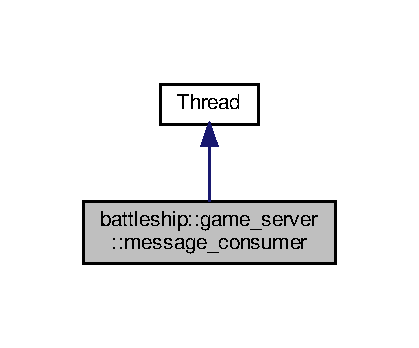
\includegraphics[width=201pt]{classbattleship_1_1game__server_1_1message__consumer__inherit__graph}
\end{center}
\end{figure}


Collaboration diagram for battleship\+:\+:game\+\_\+server\+:\+:message\+\_\+consumer\+:
\nopagebreak
\begin{figure}[H]
\begin{center}
\leavevmode
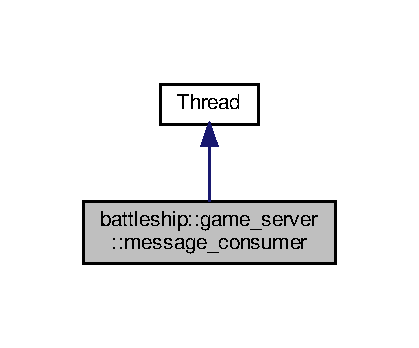
\includegraphics[width=201pt]{classbattleship_1_1game__server_1_1message__consumer__coll__graph}
\end{center}
\end{figure}
\subsection*{Public Member Functions}
\begin{DoxyCompactItemize}
\item 
\hyperlink{classbattleship_1_1game__server_1_1message__consumer_a266c52a9e282be54a95c1338432ead58}{message\+\_\+consumer} (\hyperlink{classbattleship_1_1ts__queue}{ts\+\_\+queue}$<$ \hyperlink{classbattleship_1_1network__message_1_1message}{message} $\ast$$>$ \&m\+\_\+queue, \hyperlink{classbattleship_1_1game__server_1_1client__pool}{client\+\_\+pool} \&c\+\_\+pool, \hyperlink{classbattleship_1_1game__server_1_1game__pool}{game\+\_\+pool} \&g\+\_\+pool)
\item 
void $\ast$ \hyperlink{classbattleship_1_1game__server_1_1message__consumer_ad4c9cb302cbaaa1e6c336499a218e105}{run} () override
\end{DoxyCompactItemize}


\subsection{Detailed Description}
A message consuming thread. 

\begin{DoxyAuthor}{Author}
Jonathan Henly 

Adham Kassem 
\end{DoxyAuthor}
\begin{DoxyVersion}{Version}
12-\/01-\/2018 
\end{DoxyVersion}


\subsection{Constructor \& Destructor Documentation}
\mbox{\Hypertarget{classbattleship_1_1game__server_1_1message__consumer_a266c52a9e282be54a95c1338432ead58}\label{classbattleship_1_1game__server_1_1message__consumer_a266c52a9e282be54a95c1338432ead58}} 
\index{battleship\+::game\+\_\+server\+::message\+\_\+consumer@{battleship\+::game\+\_\+server\+::message\+\_\+consumer}!message\+\_\+consumer@{message\+\_\+consumer}}
\index{message\+\_\+consumer@{message\+\_\+consumer}!battleship\+::game\+\_\+server\+::message\+\_\+consumer@{battleship\+::game\+\_\+server\+::message\+\_\+consumer}}
\subsubsection{\texorpdfstring{message\+\_\+consumer()}{message\_consumer()}}
{\footnotesize\ttfamily battleship\+::game\+\_\+server\+::message\+\_\+consumer\+::message\+\_\+consumer (\begin{DoxyParamCaption}\item[{\hyperlink{classbattleship_1_1ts__queue}{ts\+\_\+queue}$<$ \hyperlink{classbattleship_1_1network__message_1_1message}{message} $\ast$$>$ \&}]{m\+\_\+queue,  }\item[{\hyperlink{classbattleship_1_1game__server_1_1client__pool}{client\+\_\+pool} \&}]{c\+\_\+pool,  }\item[{\hyperlink{classbattleship_1_1game__server_1_1game__pool}{game\+\_\+pool} \&}]{g\+\_\+pool }\end{DoxyParamCaption})\hspace{0.3cm}{\ttfamily [inline]}}


\begin{DoxyParams}{Parameters}
{\em queue} & -\/ the thread safe message queue. \\
\hline
{\em pool} & -\/ the thread safe pool of clients. \\
\hline
{\em games} & -\/ the thread safe pool of games. \\
\hline
\end{DoxyParams}


\subsection{Member Function Documentation}
\mbox{\Hypertarget{classbattleship_1_1game__server_1_1message__consumer_ad4c9cb302cbaaa1e6c336499a218e105}\label{classbattleship_1_1game__server_1_1message__consumer_ad4c9cb302cbaaa1e6c336499a218e105}} 
\index{battleship\+::game\+\_\+server\+::message\+\_\+consumer@{battleship\+::game\+\_\+server\+::message\+\_\+consumer}!run@{run}}
\index{run@{run}!battleship\+::game\+\_\+server\+::message\+\_\+consumer@{battleship\+::game\+\_\+server\+::message\+\_\+consumer}}
\subsubsection{\texorpdfstring{run()}{run()}}
{\footnotesize\ttfamily void $\ast$ battleship\+::game\+\_\+server\+::message\+\_\+consumer\+::run (\begin{DoxyParamCaption}{ }\end{DoxyParamCaption})\hspace{0.3cm}{\ttfamily [override]}, {\ttfamily [virtual]}}

Where this
\begin{DoxyCode}
\hyperlink{classbattleship_1_1game__server_1_1message__consumer_a266c52a9e282be54a95c1338432ead58}{message\_consumer} 
\end{DoxyCode}
 thread does all of the work. 

Implements \hyperlink{classThread}{Thread}.



The documentation for this class was generated from the following files\+:\begin{DoxyCompactItemize}
\item 
inc/msgconsumer.\+h\item 
src/msgconsumer.\+cpp\end{DoxyCompactItemize}

\hypertarget{classbattleship_1_1game__server_1_1server}{}\section{battleship\+:\+:game\+\_\+server\+:\+:server Class Reference}
\label{classbattleship_1_1game__server_1_1server}\index{battleship\+::game\+\_\+server\+::server@{battleship\+::game\+\_\+server\+::server}}


Battleship server implementation that handles multiple client connections and one-\/on-\/one games.  




{\ttfamily \#include $<$server.\+h$>$}

\subsection*{Public Types}
\begin{DoxyCompactItemize}
\item 
enum \{ \hyperlink{classbattleship_1_1game__server_1_1server_a65e83301c83373edf5d10cbf6d16bf18a1ac8cde70fcc3e1fc9379b7bba6c5833}{S\+E\+R\+V\+E\+R\+\_\+\+A\+L\+R\+E\+A\+D\+Y\+\_\+\+R\+U\+N\+N\+I\+NG} = -\/1, 
\hyperlink{classbattleship_1_1game__server_1_1server_a65e83301c83373edf5d10cbf6d16bf18adbf1fba50d1b1b3e22d8e33da6266ec4}{C\+O\+U\+L\+D\+\_\+\+N\+O\+T\+\_\+\+C\+R\+E\+A\+T\+E\+\_\+\+C\+O\+N\+S\+U\+M\+E\+R\+\_\+\+T\+H\+R\+E\+A\+DS} = -\/2, 
\hyperlink{classbattleship_1_1game__server_1_1server_a65e83301c83373edf5d10cbf6d16bf18aa83ea1931d9c62e8a5f2073a01b35ed8}{C\+O\+U\+L\+D\+\_\+\+N\+O\+T\+\_\+\+C\+R\+E\+A\+T\+E\+\_\+\+C\+O\+N\+\_\+\+A\+C\+C\+E\+P\+T\+OR} = -\/3
 \}
\end{DoxyCompactItemize}
\subsection*{Public Member Functions}
\begin{DoxyCompactItemize}
\item 
\hyperlink{classbattleship_1_1game__server_1_1server_a2701536460afe0c69a7472e563041f8a}{server} (const unsigned char max\+\_\+conns, const int port, const std\+::string ip=\char`\"{}\char`\"{})
\item 
int \hyperlink{classbattleship_1_1game__server_1_1server_a07a7f97a9b7a5c1bcb0a4730a5e92745}{start} ()
\item 
\mbox{\Hypertarget{classbattleship_1_1game__server_1_1server_a396027c2491c294d4934037da1a27341}\label{classbattleship_1_1game__server_1_1server_a396027c2491c294d4934037da1a27341}} 
void {\bfseries shutdown} ()
\item 
unsigned char \hyperlink{classbattleship_1_1game__server_1_1server_a654d346dfec64a6b0563337312f0ee37}{get\+\_\+max\+\_\+connections} () const
\item 
int \hyperlink{classbattleship_1_1game__server_1_1server_afdcbafb3a745a64dc3ca05d6f4589656}{get\+\_\+port} () const
\item 
std\+::string \hyperlink{classbattleship_1_1game__server_1_1server_a877b2f81e0bcd08311f1e7c1410c9de4}{get\+\_\+ip} () const
\item 
unsigned char \hyperlink{classbattleship_1_1game__server_1_1server_a935ce9f2b8c774ff4f3904aac5c09b91}{get\+\_\+connection\+\_\+count} () const
\item 
bool \hyperlink{classbattleship_1_1game__server_1_1server_a5d740941b4dd0bd5a1773ac623b72a84}{is\+\_\+running} () const
\end{DoxyCompactItemize}


\subsection{Detailed Description}
Battleship server implementation that handles multiple client connections and one-\/on-\/one games. 

\begin{DoxyAuthor}{Author}
Adham Kassem 

Jonathan Henly 
\end{DoxyAuthor}
\begin{DoxyVersion}{Version}
11-\/27-\/2018 
\end{DoxyVersion}


\subsection{Member Enumeration Documentation}
\mbox{\Hypertarget{classbattleship_1_1game__server_1_1server_a65e83301c83373edf5d10cbf6d16bf18}\label{classbattleship_1_1game__server_1_1server_a65e83301c83373edf5d10cbf6d16bf18}} 
\subsubsection{\texorpdfstring{anonymous enum}{anonymous enum}}
{\footnotesize\ttfamily anonymous enum}

\begin{DoxyEnumFields}{Enumerator}
\raisebox{\heightof{T}}[0pt][0pt]{\index{S\+E\+R\+V\+E\+R\+\_\+\+A\+L\+R\+E\+A\+D\+Y\+\_\+\+R\+U\+N\+N\+I\+NG@{S\+E\+R\+V\+E\+R\+\_\+\+A\+L\+R\+E\+A\+D\+Y\+\_\+\+R\+U\+N\+N\+I\+NG}!battleship\+::game\+\_\+server\+::server@{battleship\+::game\+\_\+server\+::server}}\index{battleship\+::game\+\_\+server\+::server@{battleship\+::game\+\_\+server\+::server}!S\+E\+R\+V\+E\+R\+\_\+\+A\+L\+R\+E\+A\+D\+Y\+\_\+\+R\+U\+N\+N\+I\+NG@{S\+E\+R\+V\+E\+R\+\_\+\+A\+L\+R\+E\+A\+D\+Y\+\_\+\+R\+U\+N\+N\+I\+NG}}}\mbox{\Hypertarget{classbattleship_1_1game__server_1_1server_a65e83301c83373edf5d10cbf6d16bf18a1ac8cde70fcc3e1fc9379b7bba6c5833}\label{classbattleship_1_1game__server_1_1server_a65e83301c83373edf5d10cbf6d16bf18a1ac8cde70fcc3e1fc9379b7bba6c5833}} 
S\+E\+R\+V\+E\+R\+\_\+\+A\+L\+R\+E\+A\+D\+Y\+\_\+\+R\+U\+N\+N\+I\+NG&S\+E\+R\+V\+E\+R\+\_\+\+A\+L\+R\+E\+A\+D\+Y\+\_\+\+R\+U\+N\+N\+I\+NG. \\
\hline

\raisebox{\heightof{T}}[0pt][0pt]{\index{C\+O\+U\+L\+D\+\_\+\+N\+O\+T\+\_\+\+C\+R\+E\+A\+T\+E\+\_\+\+C\+O\+N\+S\+U\+M\+E\+R\+\_\+\+T\+H\+R\+E\+A\+DS@{C\+O\+U\+L\+D\+\_\+\+N\+O\+T\+\_\+\+C\+R\+E\+A\+T\+E\+\_\+\+C\+O\+N\+S\+U\+M\+E\+R\+\_\+\+T\+H\+R\+E\+A\+DS}!battleship\+::game\+\_\+server\+::server@{battleship\+::game\+\_\+server\+::server}}\index{battleship\+::game\+\_\+server\+::server@{battleship\+::game\+\_\+server\+::server}!C\+O\+U\+L\+D\+\_\+\+N\+O\+T\+\_\+\+C\+R\+E\+A\+T\+E\+\_\+\+C\+O\+N\+S\+U\+M\+E\+R\+\_\+\+T\+H\+R\+E\+A\+DS@{C\+O\+U\+L\+D\+\_\+\+N\+O\+T\+\_\+\+C\+R\+E\+A\+T\+E\+\_\+\+C\+O\+N\+S\+U\+M\+E\+R\+\_\+\+T\+H\+R\+E\+A\+DS}}}\mbox{\Hypertarget{classbattleship_1_1game__server_1_1server_a65e83301c83373edf5d10cbf6d16bf18adbf1fba50d1b1b3e22d8e33da6266ec4}\label{classbattleship_1_1game__server_1_1server_a65e83301c83373edf5d10cbf6d16bf18adbf1fba50d1b1b3e22d8e33da6266ec4}} 
C\+O\+U\+L\+D\+\_\+\+N\+O\+T\+\_\+\+C\+R\+E\+A\+T\+E\+\_\+\+C\+O\+N\+S\+U\+M\+E\+R\+\_\+\+T\+H\+R\+E\+A\+DS&C\+O\+U\+L\+D\+\_\+\+N\+O\+T\+\_\+\+C\+R\+E\+A\+T\+E\+\_\+\+C\+O\+N\+S\+U\+M\+E\+R\+\_\+\+T\+H\+R\+E\+A\+DS. \\
\hline

\raisebox{\heightof{T}}[0pt][0pt]{\index{C\+O\+U\+L\+D\+\_\+\+N\+O\+T\+\_\+\+C\+R\+E\+A\+T\+E\+\_\+\+C\+O\+N\+\_\+\+A\+C\+C\+E\+P\+T\+OR@{C\+O\+U\+L\+D\+\_\+\+N\+O\+T\+\_\+\+C\+R\+E\+A\+T\+E\+\_\+\+C\+O\+N\+\_\+\+A\+C\+C\+E\+P\+T\+OR}!battleship\+::game\+\_\+server\+::server@{battleship\+::game\+\_\+server\+::server}}\index{battleship\+::game\+\_\+server\+::server@{battleship\+::game\+\_\+server\+::server}!C\+O\+U\+L\+D\+\_\+\+N\+O\+T\+\_\+\+C\+R\+E\+A\+T\+E\+\_\+\+C\+O\+N\+\_\+\+A\+C\+C\+E\+P\+T\+OR@{C\+O\+U\+L\+D\+\_\+\+N\+O\+T\+\_\+\+C\+R\+E\+A\+T\+E\+\_\+\+C\+O\+N\+\_\+\+A\+C\+C\+E\+P\+T\+OR}}}\mbox{\Hypertarget{classbattleship_1_1game__server_1_1server_a65e83301c83373edf5d10cbf6d16bf18aa83ea1931d9c62e8a5f2073a01b35ed8}\label{classbattleship_1_1game__server_1_1server_a65e83301c83373edf5d10cbf6d16bf18aa83ea1931d9c62e8a5f2073a01b35ed8}} 
C\+O\+U\+L\+D\+\_\+\+N\+O\+T\+\_\+\+C\+R\+E\+A\+T\+E\+\_\+\+C\+O\+N\+\_\+\+A\+C\+C\+E\+P\+T\+OR&C\+O\+U\+L\+D\+\_\+\+N\+O\+T\+\_\+\+C\+R\+E\+A\+T\+E\+\_\+\+C\+O\+N\+\_\+\+A\+C\+C\+E\+P\+T\+OR. \\
\hline

\end{DoxyEnumFields}


\subsection{Constructor \& Destructor Documentation}
\mbox{\Hypertarget{classbattleship_1_1game__server_1_1server_a2701536460afe0c69a7472e563041f8a}\label{classbattleship_1_1game__server_1_1server_a2701536460afe0c69a7472e563041f8a}} 
\index{battleship\+::game\+\_\+server\+::server@{battleship\+::game\+\_\+server\+::server}!server@{server}}
\index{server@{server}!battleship\+::game\+\_\+server\+::server@{battleship\+::game\+\_\+server\+::server}}
\subsubsection{\texorpdfstring{server()}{server()}}
{\footnotesize\ttfamily battleship\+::game\+\_\+server\+::server\+::server (\begin{DoxyParamCaption}\item[{const unsigned char}]{max\+\_\+connections,  }\item[{const int}]{port,  }\item[{const std\+::string}]{ip = {\ttfamily \char`\"{}\char`\"{}} }\end{DoxyParamCaption})\hspace{0.3cm}{\ttfamily [explicit]}}


\begin{DoxyParams}{Parameters}
{\em max\+Connections} & \\
\hline
{\em port} & \\
\hline
{\em ip} & \\
\hline
\end{DoxyParams}


\subsection{Member Function Documentation}
\mbox{\Hypertarget{classbattleship_1_1game__server_1_1server_a935ce9f2b8c774ff4f3904aac5c09b91}\label{classbattleship_1_1game__server_1_1server_a935ce9f2b8c774ff4f3904aac5c09b91}} 
\index{battleship\+::game\+\_\+server\+::server@{battleship\+::game\+\_\+server\+::server}!get\+\_\+connection\+\_\+count@{get\+\_\+connection\+\_\+count}}
\index{get\+\_\+connection\+\_\+count@{get\+\_\+connection\+\_\+count}!battleship\+::game\+\_\+server\+::server@{battleship\+::game\+\_\+server\+::server}}
\subsubsection{\texorpdfstring{get\+\_\+connection\+\_\+count()}{get\_connection\_count()}}
{\footnotesize\ttfamily unsigned char battleship\+::game\+\_\+server\+::server\+::get\+\_\+connection\+\_\+count (\begin{DoxyParamCaption}{ }\end{DoxyParamCaption}) const\hspace{0.3cm}{\ttfamily [inline]}}

Gets the current number of connected clients. \begin{DoxyReturn}{Returns}
the current number of connected clients. 
\end{DoxyReturn}
\mbox{\Hypertarget{classbattleship_1_1game__server_1_1server_a877b2f81e0bcd08311f1e7c1410c9de4}\label{classbattleship_1_1game__server_1_1server_a877b2f81e0bcd08311f1e7c1410c9de4}} 
\index{battleship\+::game\+\_\+server\+::server@{battleship\+::game\+\_\+server\+::server}!get\+\_\+ip@{get\+\_\+ip}}
\index{get\+\_\+ip@{get\+\_\+ip}!battleship\+::game\+\_\+server\+::server@{battleship\+::game\+\_\+server\+::server}}
\subsubsection{\texorpdfstring{get\+\_\+ip()}{get\_ip()}}
{\footnotesize\ttfamily std\+::string battleship\+::game\+\_\+server\+::server\+::get\+\_\+ip (\begin{DoxyParamCaption}{ }\end{DoxyParamCaption}) const\hspace{0.3cm}{\ttfamily [inline]}}

Gets this server\textquotesingle{}s IP address. \begin{DoxyReturn}{Returns}
this server\textquotesingle{}s IP address. 
\end{DoxyReturn}
\mbox{\Hypertarget{classbattleship_1_1game__server_1_1server_a654d346dfec64a6b0563337312f0ee37}\label{classbattleship_1_1game__server_1_1server_a654d346dfec64a6b0563337312f0ee37}} 
\index{battleship\+::game\+\_\+server\+::server@{battleship\+::game\+\_\+server\+::server}!get\+\_\+max\+\_\+connections@{get\+\_\+max\+\_\+connections}}
\index{get\+\_\+max\+\_\+connections@{get\+\_\+max\+\_\+connections}!battleship\+::game\+\_\+server\+::server@{battleship\+::game\+\_\+server\+::server}}
\subsubsection{\texorpdfstring{get\+\_\+max\+\_\+connections()}{get\_max\_connections()}}
{\footnotesize\ttfamily unsigned char battleship\+::game\+\_\+server\+::server\+::get\+\_\+max\+\_\+connections (\begin{DoxyParamCaption}{ }\end{DoxyParamCaption}) const\hspace{0.3cm}{\ttfamily [inline]}}

Gets the maximum number of client connections for this server. \begin{DoxyReturn}{Returns}
the maximum number of client connections. 
\end{DoxyReturn}
\mbox{\Hypertarget{classbattleship_1_1game__server_1_1server_afdcbafb3a745a64dc3ca05d6f4589656}\label{classbattleship_1_1game__server_1_1server_afdcbafb3a745a64dc3ca05d6f4589656}} 
\index{battleship\+::game\+\_\+server\+::server@{battleship\+::game\+\_\+server\+::server}!get\+\_\+port@{get\+\_\+port}}
\index{get\+\_\+port@{get\+\_\+port}!battleship\+::game\+\_\+server\+::server@{battleship\+::game\+\_\+server\+::server}}
\subsubsection{\texorpdfstring{get\+\_\+port()}{get\_port()}}
{\footnotesize\ttfamily int battleship\+::game\+\_\+server\+::server\+::get\+\_\+port (\begin{DoxyParamCaption}{ }\end{DoxyParamCaption}) const\hspace{0.3cm}{\ttfamily [inline]}}

Gets the port this server is listening on. \begin{DoxyReturn}{Returns}
the port this server is listening on. 
\end{DoxyReturn}
\mbox{\Hypertarget{classbattleship_1_1game__server_1_1server_a5d740941b4dd0bd5a1773ac623b72a84}\label{classbattleship_1_1game__server_1_1server_a5d740941b4dd0bd5a1773ac623b72a84}} 
\index{battleship\+::game\+\_\+server\+::server@{battleship\+::game\+\_\+server\+::server}!is\+\_\+running@{is\+\_\+running}}
\index{is\+\_\+running@{is\+\_\+running}!battleship\+::game\+\_\+server\+::server@{battleship\+::game\+\_\+server\+::server}}
\subsubsection{\texorpdfstring{is\+\_\+running()}{is\_running()}}
{\footnotesize\ttfamily bool battleship\+::game\+\_\+server\+::server\+::is\+\_\+running (\begin{DoxyParamCaption}{ }\end{DoxyParamCaption}) const\hspace{0.3cm}{\ttfamily [inline]}}

Checks if this server is running, that is, checks whether this server is accepting connections or not. \begin{DoxyReturn}{Returns}
true if this server is running, otherwise false. 
\end{DoxyReturn}
\mbox{\Hypertarget{classbattleship_1_1game__server_1_1server_a07a7f97a9b7a5c1bcb0a4730a5e92745}\label{classbattleship_1_1game__server_1_1server_a07a7f97a9b7a5c1bcb0a4730a5e92745}} 
\index{battleship\+::game\+\_\+server\+::server@{battleship\+::game\+\_\+server\+::server}!start@{start}}
\index{start@{start}!battleship\+::game\+\_\+server\+::server@{battleship\+::game\+\_\+server\+::server}}
\subsubsection{\texorpdfstring{start()}{start()}}
{\footnotesize\ttfamily int battleship\+::game\+\_\+server\+::server\+::start (\begin{DoxyParamCaption}{ }\end{DoxyParamCaption})}

\begin{DoxyReturn}{Returns}

\end{DoxyReturn}


The documentation for this class was generated from the following files\+:\begin{DoxyCompactItemize}
\item 
inc/server.\+h\item 
src/server.\+cpp\end{DoxyCompactItemize}

\hypertarget{classtcp__acceptor}{}\section{tcp\+\_\+acceptor Class Reference}
\label{classtcp__acceptor}\index{tcp\+\_\+acceptor@{tcp\+\_\+acceptor}}
\subsection*{Public Member Functions}
\begin{DoxyCompactItemize}
\item 
\hyperlink{classtcp__acceptor_acf72994db89d547554513076de9f2e66}{tcp\+\_\+acceptor} (int port, const char $\ast$address=\char`\"{}\char`\"{})
\item 
\hyperlink{classtcp__acceptor_a8110052284976750b47ec30b900956f2}{$\sim$tcp\+\_\+acceptor} ()
\item 
int \hyperlink{classtcp__acceptor_a15116195be2fa6d2b5f432cc0bdf0479}{start} ()
\item 
\hyperlink{classtcp__stream}{tcp\+\_\+stream} $\ast$ \hyperlink{classtcp__acceptor_a44b6f54d8d69d313091d3ae8991bf696}{accept} ()
\end{DoxyCompactItemize}


\subsection{Constructor \& Destructor Documentation}
\mbox{\Hypertarget{classtcp__acceptor_acf72994db89d547554513076de9f2e66}\label{classtcp__acceptor_acf72994db89d547554513076de9f2e66}} 
\index{tcp\+\_\+acceptor@{tcp\+\_\+acceptor}!tcp\+\_\+acceptor@{tcp\+\_\+acceptor}}
\index{tcp\+\_\+acceptor@{tcp\+\_\+acceptor}!tcp\+\_\+acceptor@{tcp\+\_\+acceptor}}
\subsubsection{\texorpdfstring{tcp\+\_\+acceptor()}{tcp\_acceptor()}}
{\footnotesize\ttfamily tcp\+\_\+acceptor\+::tcp\+\_\+acceptor (\begin{DoxyParamCaption}\item[{int}]{port,  }\item[{const char $\ast$}]{address = {\ttfamily \char`\"{}\char`\"{}} }\end{DoxyParamCaption})}


\begin{DoxyParams}{Parameters}
{\em port} & \\
\hline
{\em address} & \\
\hline
\end{DoxyParams}
\mbox{\Hypertarget{classtcp__acceptor_a8110052284976750b47ec30b900956f2}\label{classtcp__acceptor_a8110052284976750b47ec30b900956f2}} 
\index{tcp\+\_\+acceptor@{tcp\+\_\+acceptor}!````~tcp\+\_\+acceptor@{$\sim$tcp\+\_\+acceptor}}
\index{````~tcp\+\_\+acceptor@{$\sim$tcp\+\_\+acceptor}!tcp\+\_\+acceptor@{tcp\+\_\+acceptor}}
\subsubsection{\texorpdfstring{$\sim$tcp\+\_\+acceptor()}{~tcp\_acceptor()}}
{\footnotesize\ttfamily tcp\+\_\+acceptor\+::$\sim$tcp\+\_\+acceptor (\begin{DoxyParamCaption}{ }\end{DoxyParamCaption})}

Closes any listening sockets. 

\subsection{Member Function Documentation}
\mbox{\Hypertarget{classtcp__acceptor_a44b6f54d8d69d313091d3ae8991bf696}\label{classtcp__acceptor_a44b6f54d8d69d313091d3ae8991bf696}} 
\index{tcp\+\_\+acceptor@{tcp\+\_\+acceptor}!accept@{accept}}
\index{accept@{accept}!tcp\+\_\+acceptor@{tcp\+\_\+acceptor}}
\subsubsection{\texorpdfstring{accept()}{accept()}}
{\footnotesize\ttfamily \hyperlink{classtcp__stream}{tcp\+\_\+stream} $\ast$ tcp\+\_\+acceptor\+::accept (\begin{DoxyParamCaption}{ }\end{DoxyParamCaption})}

\begin{DoxyReturn}{Returns}
a connection accepted by this
\begin{DoxyCode}
\hyperlink{classtcp__acceptor}{tcp\_acceptor} 
\end{DoxyCode}
 instance. 
\end{DoxyReturn}
\mbox{\Hypertarget{classtcp__acceptor_a15116195be2fa6d2b5f432cc0bdf0479}\label{classtcp__acceptor_a15116195be2fa6d2b5f432cc0bdf0479}} 
\index{tcp\+\_\+acceptor@{tcp\+\_\+acceptor}!start@{start}}
\index{start@{start}!tcp\+\_\+acceptor@{tcp\+\_\+acceptor}}
\subsubsection{\texorpdfstring{start()}{start()}}
{\footnotesize\ttfamily int tcp\+\_\+acceptor\+::start (\begin{DoxyParamCaption}{ }\end{DoxyParamCaption})}

Start listening for connections with this
\begin{DoxyCode}
\hyperlink{classtcp__acceptor}{tcp\_acceptor} 
\end{DoxyCode}
 instance.

\begin{DoxyReturn}{Returns}
0 on successful start, non-\/zero if an error occurred. 
\end{DoxyReturn}


The documentation for this class was generated from the following files\+:\begin{DoxyCompactItemize}
\item 
shared/inc/tcpacceptor.\+h\item 
shared/src/tcpacceptor.\+cpp\end{DoxyCompactItemize}

\hypertarget{classtcp__connector}{}\section{tcp\+\_\+connector Class Reference}
\label{classtcp__connector}\index{tcp\+\_\+connector@{tcp\+\_\+connector}}


To\+Do document this class.  




{\ttfamily \#include $<$tcpconnector.\+h$>$}

\subsection*{Public Member Functions}
\begin{DoxyCompactItemize}
\item 
\hyperlink{classtcp__stream}{tcp\+\_\+stream} $\ast$ \hyperlink{classtcp__connector_a1f542ff6507a639154099b4c2dafb729}{connect} (const char $\ast$server, const int port, const int tout\+\_\+s=0, const int tout\+\_\+us=0)
\end{DoxyCompactItemize}


\subsection{Detailed Description}
To\+Do document this class. 

\begin{DoxyAuthor}{Author}
Jonathan Henly 

Adham Kassem 
\end{DoxyAuthor}
\begin{DoxyVersion}{Version}
11-\/27-\/2018 
\end{DoxyVersion}


\subsection{Member Function Documentation}
\mbox{\Hypertarget{classtcp__connector_a1f542ff6507a639154099b4c2dafb729}\label{classtcp__connector_a1f542ff6507a639154099b4c2dafb729}} 
\index{tcp\+\_\+connector@{tcp\+\_\+connector}!connect@{connect}}
\index{connect@{connect}!tcp\+\_\+connector@{tcp\+\_\+connector}}
\subsubsection{\texorpdfstring{connect()}{connect()}}
{\footnotesize\ttfamily \hyperlink{classtcp__stream}{tcp\+\_\+stream} $\ast$ tcp\+\_\+connector\+::connect (\begin{DoxyParamCaption}\item[{const char $\ast$}]{server,  }\item[{const int}]{port,  }\item[{const int}]{tout\+\_\+s = {\ttfamily 0},  }\item[{const int}]{tout\+\_\+us = {\ttfamily 0} }\end{DoxyParamCaption})}

To\+Do document this method


\begin{DoxyParams}{Parameters}
{\em server} & \\
\hline
{\em port} & \\
\hline
\end{DoxyParams}
\begin{DoxyReturn}{Returns}

\end{DoxyReturn}


The documentation for this class was generated from the following files\+:\begin{DoxyCompactItemize}
\item 
shared/inc/tcpconnector.\+h\item 
shared/src/tcpconnector.\+cpp\end{DoxyCompactItemize}

\hypertarget{classtcp__stream}{}\section{tcp\+\_\+stream Class Reference}
\label{classtcp__stream}\index{tcp\+\_\+stream@{tcp\+\_\+stream}}


{\ttfamily \#include $<$tcpstream.\+h$>$}

\subsection*{Public Types}
\begin{DoxyCompactItemize}
\item 
enum \hyperlink{classtcp__stream_a1654b581bd89eacae6c5c00bf44bd303}{stream\+\_\+error} \{ \hyperlink{classtcp__stream_a1654b581bd89eacae6c5c00bf44bd303af56262b6dafb79a22137a3459fc8e6c1}{C\+O\+N\+N\+E\+C\+T\+I\+O\+N\+\_\+\+C\+L\+O\+S\+ED} = 0, 
\hyperlink{classtcp__stream_a1654b581bd89eacae6c5c00bf44bd303ab63bfd071e8d91d93ef8723b79563f0e}{C\+O\+N\+N\+E\+C\+T\+I\+O\+N\+\_\+\+T\+I\+M\+E\+O\+UT} = -\/1, 
\hyperlink{classtcp__stream_a1654b581bd89eacae6c5c00bf44bd303a4d1f1bf6e8aa323d3de6ab6254af5e1c}{C\+O\+N\+N\+E\+C\+T\+I\+O\+N\+\_\+\+R\+E\+S\+ET} = -\/2
 \}
\end{DoxyCompactItemize}
\subsection*{Public Member Functions}
\begin{DoxyCompactItemize}
\item 
\hyperlink{classtcp__stream_a5053337af64329d01e1c78cca9d5633e}{$\sim$tcp\+\_\+stream} ()
\item 
ssize\+\_\+t \hyperlink{classtcp__stream_a647c576fed72122b5dc3b6e23c36e210}{send} (const char $\ast$buffer, const size\+\_\+t len)
\item 
ssize\+\_\+t \hyperlink{classtcp__stream_a061ef2188c1cf0eebc7290dbc908f06e}{receive} (char $\ast$buffer, const size\+\_\+t len, const int tout\+\_\+s=0, const int tout\+\_\+us=0)
\item 
std\+::string \hyperlink{classtcp__stream_ac9afe2de961bc45ffb1b614e5718b353}{get\+\_\+peer\+\_\+ip} () const
\item 
int \hyperlink{classtcp__stream_a5562bfad5ec43e358b6bc63386166a50}{get\+\_\+peer\+\_\+port} () const
\end{DoxyCompactItemize}
\subsection*{Friends}
\begin{DoxyCompactItemize}
\item 
\mbox{\Hypertarget{classtcp__stream_ac753a6c4530e663615a7b160569a446f}\label{classtcp__stream_ac753a6c4530e663615a7b160569a446f}} 
class {\bfseries tcp\+\_\+acceptor}
\item 
\mbox{\Hypertarget{classtcp__stream_a35780d6902edba55e3d463e00117657d}\label{classtcp__stream_a35780d6902edba55e3d463e00117657d}} 
class {\bfseries tcp\+\_\+connector}
\end{DoxyCompactItemize}


\subsection{Detailed Description}
The \hyperlink{classtcp__stream}{tcp\+\_\+stream} class provides methods to transfer data between peers over a T\+C\+P/\+IP connection.

To\+Do give attribution to original source of T\+CP classes

\begin{DoxyAuthor}{Author}
Jonathan Henly 

Adham Kassem 
\end{DoxyAuthor}
\begin{DoxyVersion}{Version}
11-\/25-\/2018 
\end{DoxyVersion}


\subsection{Member Enumeration Documentation}
\mbox{\Hypertarget{classtcp__stream_a1654b581bd89eacae6c5c00bf44bd303}\label{classtcp__stream_a1654b581bd89eacae6c5c00bf44bd303}} 
\index{tcp\+\_\+stream@{tcp\+\_\+stream}!stream\+\_\+error@{stream\+\_\+error}}
\index{stream\+\_\+error@{stream\+\_\+error}!tcp\+\_\+stream@{tcp\+\_\+stream}}
\subsubsection{\texorpdfstring{stream\+\_\+error}{stream\_error}}
{\footnotesize\ttfamily enum \hyperlink{classtcp__stream_a1654b581bd89eacae6c5c00bf44bd303}{tcp\+\_\+stream\+::stream\+\_\+error}}

\begin{DoxyEnumFields}{Enumerator}
\raisebox{\heightof{T}}[0pt][0pt]{\index{C\+O\+N\+N\+E\+C\+T\+I\+O\+N\+\_\+\+C\+L\+O\+S\+ED@{C\+O\+N\+N\+E\+C\+T\+I\+O\+N\+\_\+\+C\+L\+O\+S\+ED}!tcp\+\_\+stream@{tcp\+\_\+stream}}\index{tcp\+\_\+stream@{tcp\+\_\+stream}!C\+O\+N\+N\+E\+C\+T\+I\+O\+N\+\_\+\+C\+L\+O\+S\+ED@{C\+O\+N\+N\+E\+C\+T\+I\+O\+N\+\_\+\+C\+L\+O\+S\+ED}}}\mbox{\Hypertarget{classtcp__stream_a1654b581bd89eacae6c5c00bf44bd303af56262b6dafb79a22137a3459fc8e6c1}\label{classtcp__stream_a1654b581bd89eacae6c5c00bf44bd303af56262b6dafb79a22137a3459fc8e6c1}} 
C\+O\+N\+N\+E\+C\+T\+I\+O\+N\+\_\+\+C\+L\+O\+S\+ED&C\+O\+N\+N\+E\+C\+T\+I\+O\+N\+\_\+\+C\+L\+O\+S\+ED. \\
\hline

\raisebox{\heightof{T}}[0pt][0pt]{\index{C\+O\+N\+N\+E\+C\+T\+I\+O\+N\+\_\+\+T\+I\+M\+E\+O\+UT@{C\+O\+N\+N\+E\+C\+T\+I\+O\+N\+\_\+\+T\+I\+M\+E\+O\+UT}!tcp\+\_\+stream@{tcp\+\_\+stream}}\index{tcp\+\_\+stream@{tcp\+\_\+stream}!C\+O\+N\+N\+E\+C\+T\+I\+O\+N\+\_\+\+T\+I\+M\+E\+O\+UT@{C\+O\+N\+N\+E\+C\+T\+I\+O\+N\+\_\+\+T\+I\+M\+E\+O\+UT}}}\mbox{\Hypertarget{classtcp__stream_a1654b581bd89eacae6c5c00bf44bd303ab63bfd071e8d91d93ef8723b79563f0e}\label{classtcp__stream_a1654b581bd89eacae6c5c00bf44bd303ab63bfd071e8d91d93ef8723b79563f0e}} 
C\+O\+N\+N\+E\+C\+T\+I\+O\+N\+\_\+\+T\+I\+M\+E\+O\+UT&C\+O\+N\+N\+E\+C\+T\+I\+O\+N\+\_\+\+T\+I\+M\+E\+D\+O\+UT. \\
\hline

\raisebox{\heightof{T}}[0pt][0pt]{\index{C\+O\+N\+N\+E\+C\+T\+I\+O\+N\+\_\+\+R\+E\+S\+ET@{C\+O\+N\+N\+E\+C\+T\+I\+O\+N\+\_\+\+R\+E\+S\+ET}!tcp\+\_\+stream@{tcp\+\_\+stream}}\index{tcp\+\_\+stream@{tcp\+\_\+stream}!C\+O\+N\+N\+E\+C\+T\+I\+O\+N\+\_\+\+R\+E\+S\+ET@{C\+O\+N\+N\+E\+C\+T\+I\+O\+N\+\_\+\+R\+E\+S\+ET}}}\mbox{\Hypertarget{classtcp__stream_a1654b581bd89eacae6c5c00bf44bd303a4d1f1bf6e8aa323d3de6ab6254af5e1c}\label{classtcp__stream_a1654b581bd89eacae6c5c00bf44bd303a4d1f1bf6e8aa323d3de6ab6254af5e1c}} 
C\+O\+N\+N\+E\+C\+T\+I\+O\+N\+\_\+\+R\+E\+S\+ET&C\+O\+N\+N\+E\+C\+T\+I\+O\+N\+\_\+\+R\+E\+S\+ET. \\
\hline

\end{DoxyEnumFields}


\subsection{Constructor \& Destructor Documentation}
\mbox{\Hypertarget{classtcp__stream_a5053337af64329d01e1c78cca9d5633e}\label{classtcp__stream_a5053337af64329d01e1c78cca9d5633e}} 
\index{tcp\+\_\+stream@{tcp\+\_\+stream}!````~tcp\+\_\+stream@{$\sim$tcp\+\_\+stream}}
\index{````~tcp\+\_\+stream@{$\sim$tcp\+\_\+stream}!tcp\+\_\+stream@{tcp\+\_\+stream}}
\subsubsection{\texorpdfstring{$\sim$tcp\+\_\+stream()}{~tcp\_stream()}}
{\footnotesize\ttfamily tcp\+\_\+stream\+::$\sim$tcp\+\_\+stream (\begin{DoxyParamCaption}{ }\end{DoxyParamCaption})}

Destructor that closes the socket descriptor associated with this T\+CP stream. 

\subsection{Member Function Documentation}
\mbox{\Hypertarget{classtcp__stream_ac9afe2de961bc45ffb1b614e5718b353}\label{classtcp__stream_ac9afe2de961bc45ffb1b614e5718b353}} 
\index{tcp\+\_\+stream@{tcp\+\_\+stream}!get\+\_\+peer\+\_\+ip@{get\+\_\+peer\+\_\+ip}}
\index{get\+\_\+peer\+\_\+ip@{get\+\_\+peer\+\_\+ip}!tcp\+\_\+stream@{tcp\+\_\+stream}}
\subsubsection{\texorpdfstring{get\+\_\+peer\+\_\+ip()}{get\_peer\_ip()}}
{\footnotesize\ttfamily std\+::string tcp\+\_\+stream\+::get\+\_\+peer\+\_\+ip (\begin{DoxyParamCaption}{ }\end{DoxyParamCaption}) const}

\begin{DoxyReturn}{Returns}
the IP address this stream is connected to. 
\end{DoxyReturn}
\mbox{\Hypertarget{classtcp__stream_a5562bfad5ec43e358b6bc63386166a50}\label{classtcp__stream_a5562bfad5ec43e358b6bc63386166a50}} 
\index{tcp\+\_\+stream@{tcp\+\_\+stream}!get\+\_\+peer\+\_\+port@{get\+\_\+peer\+\_\+port}}
\index{get\+\_\+peer\+\_\+port@{get\+\_\+peer\+\_\+port}!tcp\+\_\+stream@{tcp\+\_\+stream}}
\subsubsection{\texorpdfstring{get\+\_\+peer\+\_\+port()}{get\_peer\_port()}}
{\footnotesize\ttfamily int tcp\+\_\+stream\+::get\+\_\+peer\+\_\+port (\begin{DoxyParamCaption}{ }\end{DoxyParamCaption}) const}

\begin{DoxyReturn}{Returns}
the port this stream is connected to. 
\end{DoxyReturn}
\mbox{\Hypertarget{classtcp__stream_a061ef2188c1cf0eebc7290dbc908f06e}\label{classtcp__stream_a061ef2188c1cf0eebc7290dbc908f06e}} 
\index{tcp\+\_\+stream@{tcp\+\_\+stream}!receive@{receive}}
\index{receive@{receive}!tcp\+\_\+stream@{tcp\+\_\+stream}}
\subsubsection{\texorpdfstring{receive()}{receive()}}
{\footnotesize\ttfamily ssize\+\_\+t tcp\+\_\+stream\+::receive (\begin{DoxyParamCaption}\item[{char $\ast$}]{buffer,  }\item[{const size\+\_\+t}]{len,  }\item[{const int}]{tout\+\_\+s = {\ttfamily 0},  }\item[{const int}]{tout\+\_\+us = {\ttfamily 0} }\end{DoxyParamCaption})}


\begin{DoxyParams}{Parameters}
{\em buffer} & -\/ a pointer to a char arrays to store the read in bytes. \\
\hline
{\em len} & -\/ the number of bytes to read into buffer. \\
\hline
{\em tout\+\_\+s} & -\/ timeout in seconds, default is 0. \\
\hline
{\em tout\+\_\+us} & -\/ timeout in microseconds, default is 0. \\
\hline
\end{DoxyParams}
\begin{DoxyReturn}{Returns}

\end{DoxyReturn}
\mbox{\Hypertarget{classtcp__stream_a647c576fed72122b5dc3b6e23c36e210}\label{classtcp__stream_a647c576fed72122b5dc3b6e23c36e210}} 
\index{tcp\+\_\+stream@{tcp\+\_\+stream}!send@{send}}
\index{send@{send}!tcp\+\_\+stream@{tcp\+\_\+stream}}
\subsubsection{\texorpdfstring{send()}{send()}}
{\footnotesize\ttfamily ssize\+\_\+t tcp\+\_\+stream\+::send (\begin{DoxyParamCaption}\item[{const char $\ast$}]{buffer,  }\item[{const size\+\_\+t}]{len }\end{DoxyParamCaption})}


\begin{DoxyParams}{Parameters}
{\em buffer} & \\
\hline
{\em len} & \\
\hline
\end{DoxyParams}
\begin{DoxyReturn}{Returns}

\end{DoxyReturn}


The documentation for this class was generated from the following files\+:\begin{DoxyCompactItemize}
\item 
shared/inc/tcpstream.\+h\item 
shared/src/tcpstream.\+cpp\end{DoxyCompactItemize}

\hypertarget{classThread}{}\section{Thread Class Reference}
\label{classThread}\index{Thread@{Thread}}


A pthread wrapper implementation.  




{\ttfamily \#include $<$thread.\+h$>$}



Inheritance diagram for Thread\+:
\nopagebreak
\begin{figure}[H]
\begin{center}
\leavevmode
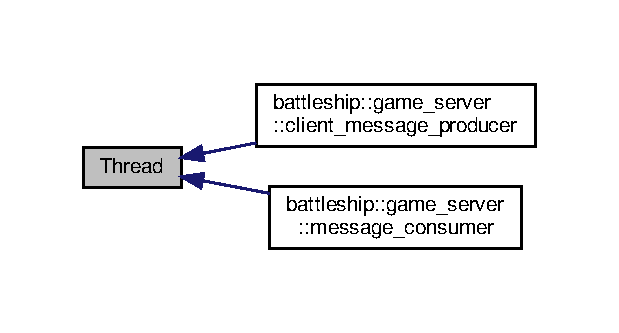
\includegraphics[width=297pt]{classThread__inherit__graph}
\end{center}
\end{figure}
\subsection*{Public Member Functions}
\begin{DoxyCompactItemize}
\item 
\hyperlink{classThread_a95c703fb8f2f27cb64f475a8c940864a}{Thread} ()
\item 
virtual \hyperlink{classThread_a37d9edd3a1a776cbc27dedff949c9726}{$\sim$\+Thread} ()
\item 
int \hyperlink{classThread_a7d563f3201d081af8cc24ea552c6a4e4}{start} ()
\item 
int \hyperlink{classThread_a7c3b04b32b4327923cc4c9553a403e32}{join} ()
\item 
int \hyperlink{classThread_a2a08036a4598cfc554114fee9d0e8485}{detach} ()
\item 
pthread\+\_\+t \hyperlink{classThread_ad4242a739c70bd1fe6b9c6e208714310}{self} ()
\item 
\mbox{\Hypertarget{classThread_a0ceaa28981eacf1051845542053d82b6}\label{classThread_a0ceaa28981eacf1051845542053d82b6}} 
virtual void $\ast$ {\bfseries run} ()=0
\end{DoxyCompactItemize}


\subsection{Detailed Description}
A pthread wrapper implementation. 

\begin{DoxyAuthor}{Author}
Jonathan Henly 

Adham Kassem 
\end{DoxyAuthor}
\begin{DoxyVersion}{Version}
11-\/27-\/2018 
\end{DoxyVersion}


\subsection{Constructor \& Destructor Documentation}
\mbox{\Hypertarget{classThread_a95c703fb8f2f27cb64f475a8c940864a}\label{classThread_a95c703fb8f2f27cb64f475a8c940864a}} 
\index{Thread@{Thread}!Thread@{Thread}}
\index{Thread@{Thread}!Thread@{Thread}}
\subsubsection{\texorpdfstring{Thread()}{Thread()}}
{\footnotesize\ttfamily Thread\+::\+Thread (\begin{DoxyParamCaption}{ }\end{DoxyParamCaption})}

To\+Do document \mbox{\Hypertarget{classThread_a37d9edd3a1a776cbc27dedff949c9726}\label{classThread_a37d9edd3a1a776cbc27dedff949c9726}} 
\index{Thread@{Thread}!````~Thread@{$\sim$\+Thread}}
\index{````~Thread@{$\sim$\+Thread}!Thread@{Thread}}
\subsubsection{\texorpdfstring{$\sim$\+Thread()}{~Thread()}}
{\footnotesize\ttfamily Thread\+::$\sim$\+Thread (\begin{DoxyParamCaption}{ }\end{DoxyParamCaption})\hspace{0.3cm}{\ttfamily [virtual]}}

To\+Do document 

\subsection{Member Function Documentation}
\mbox{\Hypertarget{classThread_a2a08036a4598cfc554114fee9d0e8485}\label{classThread_a2a08036a4598cfc554114fee9d0e8485}} 
\index{Thread@{Thread}!detach@{detach}}
\index{detach@{detach}!Thread@{Thread}}
\subsubsection{\texorpdfstring{detach()}{detach()}}
{\footnotesize\ttfamily int Thread\+::detach (\begin{DoxyParamCaption}{ }\end{DoxyParamCaption})}

Separates the thread of execution from the thread object, allowing execution to continue independently. \begin{DoxyReturn}{Returns}
0 if this thread detaches, otherwise a non-\/zero value. 
\end{DoxyReturn}
\mbox{\Hypertarget{classThread_a7c3b04b32b4327923cc4c9553a403e32}\label{classThread_a7c3b04b32b4327923cc4c9553a403e32}} 
\index{Thread@{Thread}!join@{join}}
\index{join@{join}!Thread@{Thread}}
\subsubsection{\texorpdfstring{join()}{join()}}
{\footnotesize\ttfamily int Thread\+::join (\begin{DoxyParamCaption}{ }\end{DoxyParamCaption})}

Blocks the current thread until this thread finishes its execution. \begin{DoxyReturn}{Returns}
0 if this thread joins, otherwise a non-\/zero value. 
\end{DoxyReturn}
\mbox{\Hypertarget{classThread_ad4242a739c70bd1fe6b9c6e208714310}\label{classThread_ad4242a739c70bd1fe6b9c6e208714310}} 
\index{Thread@{Thread}!self@{self}}
\index{self@{self}!Thread@{Thread}}
\subsubsection{\texorpdfstring{self()}{self()}}
{\footnotesize\ttfamily pthread\+\_\+t Thread\+::self (\begin{DoxyParamCaption}{ }\end{DoxyParamCaption})}

\begin{DoxyReturn}{Returns}
this thread\textquotesingle{}s id. 
\end{DoxyReturn}
\mbox{\Hypertarget{classThread_a7d563f3201d081af8cc24ea552c6a4e4}\label{classThread_a7d563f3201d081af8cc24ea552c6a4e4}} 
\index{Thread@{Thread}!start@{start}}
\index{start@{start}!Thread@{Thread}}
\subsubsection{\texorpdfstring{start()}{start()}}
{\footnotesize\ttfamily int Thread\+::start (\begin{DoxyParamCaption}{ }\end{DoxyParamCaption})}

\begin{DoxyReturn}{Returns}
0 if this thread successfully starts, otherwise a non-\/zero value. 
\end{DoxyReturn}


The documentation for this class was generated from the following files\+:\begin{DoxyCompactItemize}
\item 
inc/thread.\+h\item 
src/thread.\+cpp\end{DoxyCompactItemize}

\hypertarget{classbattleship_1_1ts__queue}{}\section{battleship\+:\+:ts\+\_\+queue$<$ T $>$ Class Template Reference}
\label{classbattleship_1_1ts__queue}\index{battleship\+::ts\+\_\+queue$<$ T $>$@{battleship\+::ts\+\_\+queue$<$ T $>$}}


A thread safe queue implementation.  




{\ttfamily \#include $<$tsqueue.\+h$>$}

\subsection*{Public Member Functions}
\begin{DoxyCompactItemize}
\item 
\hyperlink{classbattleship_1_1ts__queue_a8c5d650bd3c8da2226a93ef16eddf259}{ts\+\_\+queue} ()
\item 
\hyperlink{classbattleship_1_1ts__queue_ad1dcfe27a6218886353c17c9334a4232}{$\sim$ts\+\_\+queue} ()
\item 
void \hyperlink{classbattleship_1_1ts__queue_accbd5de0ef9994e7b99f2e9113a36677}{add} (T item)
\item 
T \hyperlink{classbattleship_1_1ts__queue_aa6ec6739ad7f1768068cb1f7d5957b2f}{remove} ()
\item 
size\+\_\+t \hyperlink{classbattleship_1_1ts__queue_a45ee4b66d4e5da270559887775659c6f}{size} ()
\end{DoxyCompactItemize}


\subsection{Detailed Description}
\subsubsection*{template$<$typename T$>$\newline
class battleship\+::ts\+\_\+queue$<$ T $>$}

A thread safe queue implementation. 

\begin{DoxyAuthor}{Author}
Jonathan Henly 

Adham Kassem 
\end{DoxyAuthor}
\begin{DoxyVersion}{Version}
12-\/3-\/2018 
\end{DoxyVersion}


\subsection{Constructor \& Destructor Documentation}
\mbox{\Hypertarget{classbattleship_1_1ts__queue_a8c5d650bd3c8da2226a93ef16eddf259}\label{classbattleship_1_1ts__queue_a8c5d650bd3c8da2226a93ef16eddf259}} 
\index{battleship\+::ts\+\_\+queue@{battleship\+::ts\+\_\+queue}!ts\+\_\+queue@{ts\+\_\+queue}}
\index{ts\+\_\+queue@{ts\+\_\+queue}!battleship\+::ts\+\_\+queue@{battleship\+::ts\+\_\+queue}}
\subsubsection{\texorpdfstring{ts\+\_\+queue()}{ts\_queue()}}
{\footnotesize\ttfamily template$<$typename T$>$ \\
\hyperlink{classbattleship_1_1ts__queue}{battleship\+::ts\+\_\+queue}$<$ T $>$\+::\hyperlink{classbattleship_1_1ts__queue}{ts\+\_\+queue} (\begin{DoxyParamCaption}{ }\end{DoxyParamCaption})\hspace{0.3cm}{\ttfamily [inline]}}

Default constructor. \mbox{\Hypertarget{classbattleship_1_1ts__queue_ad1dcfe27a6218886353c17c9334a4232}\label{classbattleship_1_1ts__queue_ad1dcfe27a6218886353c17c9334a4232}} 
\index{battleship\+::ts\+\_\+queue@{battleship\+::ts\+\_\+queue}!````~ts\+\_\+queue@{$\sim$ts\+\_\+queue}}
\index{````~ts\+\_\+queue@{$\sim$ts\+\_\+queue}!battleship\+::ts\+\_\+queue@{battleship\+::ts\+\_\+queue}}
\subsubsection{\texorpdfstring{$\sim$ts\+\_\+queue()}{~ts\_queue()}}
{\footnotesize\ttfamily template$<$typename T$>$ \\
\hyperlink{classbattleship_1_1ts__queue}{battleship\+::ts\+\_\+queue}$<$ T $>$\+::$\sim$\hyperlink{classbattleship_1_1ts__queue}{ts\+\_\+queue} (\begin{DoxyParamCaption}{ }\end{DoxyParamCaption})\hspace{0.3cm}{\ttfamily [inline]}}

Default destructor. 

\subsection{Member Function Documentation}
\mbox{\Hypertarget{classbattleship_1_1ts__queue_accbd5de0ef9994e7b99f2e9113a36677}\label{classbattleship_1_1ts__queue_accbd5de0ef9994e7b99f2e9113a36677}} 
\index{battleship\+::ts\+\_\+queue@{battleship\+::ts\+\_\+queue}!add@{add}}
\index{add@{add}!battleship\+::ts\+\_\+queue@{battleship\+::ts\+\_\+queue}}
\subsubsection{\texorpdfstring{add()}{add()}}
{\footnotesize\ttfamily template$<$typename T$>$ \\
void \hyperlink{classbattleship_1_1ts__queue}{battleship\+::ts\+\_\+queue}$<$ T $>$\+::add (\begin{DoxyParamCaption}\item[{T}]{item }\end{DoxyParamCaption})\hspace{0.3cm}{\ttfamily [inline]}}

\hyperlink{classThread}{Thread} safe method that adds a passed in item to the end of this queue.


\begin{DoxyParams}{Parameters}
{\em item} & -\/ the item to add to the end of the queue. \\
\hline
\end{DoxyParams}
\mbox{\Hypertarget{classbattleship_1_1ts__queue_aa6ec6739ad7f1768068cb1f7d5957b2f}\label{classbattleship_1_1ts__queue_aa6ec6739ad7f1768068cb1f7d5957b2f}} 
\index{battleship\+::ts\+\_\+queue@{battleship\+::ts\+\_\+queue}!remove@{remove}}
\index{remove@{remove}!battleship\+::ts\+\_\+queue@{battleship\+::ts\+\_\+queue}}
\subsubsection{\texorpdfstring{remove()}{remove()}}
{\footnotesize\ttfamily template$<$typename T$>$ \\
T \hyperlink{classbattleship_1_1ts__queue}{battleship\+::ts\+\_\+queue}$<$ T $>$\+::remove (\begin{DoxyParamCaption}{ }\end{DoxyParamCaption})\hspace{0.3cm}{\ttfamily [inline]}}

\hyperlink{classThread}{Thread} safe remove method that pops and returns the front of this queue. If the queue is empty, then this method will block until the queue is not empty.

\begin{DoxyReturn}{Returns}
the item at the front of the queue. 
\end{DoxyReturn}
\mbox{\Hypertarget{classbattleship_1_1ts__queue_a45ee4b66d4e5da270559887775659c6f}\label{classbattleship_1_1ts__queue_a45ee4b66d4e5da270559887775659c6f}} 
\index{battleship\+::ts\+\_\+queue@{battleship\+::ts\+\_\+queue}!size@{size}}
\index{size@{size}!battleship\+::ts\+\_\+queue@{battleship\+::ts\+\_\+queue}}
\subsubsection{\texorpdfstring{size()}{size()}}
{\footnotesize\ttfamily template$<$typename T$>$ \\
size\+\_\+t \hyperlink{classbattleship_1_1ts__queue}{battleship\+::ts\+\_\+queue}$<$ T $>$\+::size (\begin{DoxyParamCaption}{ }\end{DoxyParamCaption})\hspace{0.3cm}{\ttfamily [inline]}}

\hyperlink{classThread}{Thread} safe method that gets the size of this queue.

\begin{DoxyReturn}{Returns}
the size of this queue. 
\end{DoxyReturn}


The documentation for this class was generated from the following file\+:\begin{DoxyCompactItemize}
\item 
inc/tsqueue.\+h\end{DoxyCompactItemize}

%--- End generated contents ---

% Index
\backmatter
\newpage
\phantomsection
\clearemptydoublepage
\addcontentsline{toc}{chapter}{Index}
\printindex

\end{document}
